\documentclass[11pt]{article}

% Change "review" to "final" to generate the final (camera-ready) version.
\usepackage[review]{acl}

% Standard package includes
\usepackage{times}
\usepackage{latexsym}
\usepackage[T1]{fontenc}
\usepackage[utf8]{inputenc}
\usepackage{microtype}
\setlength{\emergencystretch}{2em}
\usepackage{inconsolata}
\usepackage{graphicx}
\usepackage{booktabs}
\usepackage{multirow}
\usepackage{tabularx}
\usepackage{fvextra}
\usepackage{amssymb}
\DefineVerbatimEnvironment{SPARQL}{Verbatim}{breaklines=true,breakanywhere=true,fontsize=\small}

\title{PIPE-RDF: Execution-Grounded Generation of Schema-Specific NL--SPARQL Benchmarks}

\author{
  Anonymous Author(s) \\
  Anonymous Affiliation \\
  Anonymous Address \\
  \texttt{anonymous@anonymous.edu}
}

\begin{document}
\maketitle

\begin{abstract}
Natural-language interfaces to Resource Description Framework (RDF) knowledge graphs require benchmarks whose SPARQL queries match the target schema, namespace conventions, and query distribution. Public knowledge-graph question answering (KGQA) datasets are useful for model comparison, but they are not designed to create evaluation sets for a new RDF schema. We present PIPE-RDF, a three-phase pipeline for constructing schema-specific natural-language--SPARQL (NL--SPARQL) benchmarks using reverse querying, category-balanced template generation, retrieval-augmented prompting, deduplication, and execution-based validation. We evaluate PIPE-RDF on two RDF schemas: a controlled company-location slice and a broader 25M-triple LDBC Semantic Publishing Benchmark (SPB) graph. The primary Qwen3.5-4B runs generate 3{,}600 Phase-3 pairs, exactly 200 per category for each schema across nine categories, with 100\% parse validity, 100\% execution validity, zero empty answers, and zero repairs under strict acceptance. Six cross-model probes with Qwen3.5-2B, 4B, and 9B produce balanced 450-pair benchmarks on both schemas with the same strict validity profile. A downstream utility study shows that category-retrieval prompting with generated examples substantially improves NL-to-SPARQL execution and answer accuracy over schema-only zero-shot prompting. Code is available at \url{https://anonymous.4open.science/status/PIPE-RDF-B750}.
\end{abstract}

\section{Introduction}
RDF knowledge graphs expose structured data through SPARQL, but natural-language access to those graphs remains highly schema-dependent. A natural-language question can be fluent while its corresponding query uses the wrong predicate, assumes a missing type, or returns an answer set that cannot exist in the target graph. This makes benchmark construction a first-order problem for NL--SPARQL work: an evaluation set must reflect the target ontology, prefixes, available attributes, and intended query categories before it can be used to compare parsers or retrieval strategies.

Public KGQA benchmarks such as LC-QuAD, QALD-9-plus, and Mintaka provide valuable shared test beds, but they are tied to fixed public schemas and entity distributions \citep{Trivedi_2017,perevalov2022qald9plusmultilingualdatasetquestion,sen2022mintakacomplexnaturalmultilingual}. They do not directly answer a common methodological question: given a new RDF schema, how can we construct a balanced, executable, and auditable NL--SPARQL benchmark without manually authoring every query? Modern large language models (LLMs) can help generate candidate questions and queries \citep{brown2020languagemodelsfewshotlearners,touvron2023llamaopenefficientfoundation}, but unconstrained generation is prone to unsupported entities, invalid predicates, and semantically plausible but unanswerable queries.

PIPE-RDF addresses this benchmark-construction problem with a pipeline that grounds generation in graph facts. The central mechanism is reverse querying: before a question--query pair is accepted, the system first finds entity bindings that satisfy the intended template in the target graph. Category-balanced generation, retrieval-augmented prompting, predicate/type whitelists, deduplication, execution validation, and repair are then used to produce benchmark artifacts that are not merely grammatical, but executable against a fixed RDF endpoint.

\textbf{Contributions.} We:
\begin{itemize}
  \item propose a three-phase pipeline for schema-specific NL--SPARQL benchmark generation with reverse-query grounding and execution validation;
  \item evaluate PIPE-RDF on a fixed company-location schema and a broader LDBC Semantic Publishing Benchmark (SPB) graph, producing 3{,}600 strictly valid Phase-3 pairs across nine categories;
  \item report operational metrics including parse validity, execution success, empty-result rates, repair rates, latency, strategy coverage, and entity diversity;
  \item add cross-model robustness probes and a compact downstream utility evaluation for zero-shot versus retrieval-augmented NL-to-SPARQL prompting;
  \item provide a stratified semantic-audit packet and agreement tooling for independent human validation.
\end{itemize}

\section{Background and Related Work}
\textbf{Benchmark coverage and query taxonomies.} KGQA benchmarks often over-represent simple factoid queries. Mintaka explicitly balances query categories (counting, comparative, superlative, ordinal, multi-hop, intersection, difference/negation, yes/no, and generic) to avoid skewed evaluation \citep{sen2022mintakacomplexnaturalmultilingual}. Public datasets such as LC-QuAD and QALD-9-plus provide valuable coverage but remain tied to public graphs and fixed schemas \citep{Trivedi_2017,perevalov2022qald9plusmultilingualdatasetquestion}. Dynamic benchmarking efforts such as Dynabench further highlight the need for iterative, real-world evaluation \citep{kiela2021dynabenchrethinkingbenchmarkingnlp}.

\textbf{Retrieval augmentation and prompting.} Retrieval-augmented generation (RAG) improves text-to-query performance by conditioning on relevant examples and schema cues \citep{lewis2021retrievalaugmentedgenerationknowledgeintensivenlp}. In practice, RAG offers a low-cost alternative to fine-tuning when schema-specific examples are scarce. PIPE-RDF maintains category-specific retrieval banks to provide structurally similar NL--SPARQL pairs during generation, reducing cross-category drift and improving template grounding.

\textbf{Validity and evaluation.} Grammar-constrained decoding (e.g., PICARD) improves syntactic correctness for structured query generation \citep{Scholak_2021}. SPARQL-specific metrics such as SP-BLEU/SP-F1 normalize variables for fairer matching \citep{Rony_2022}, while code-oriented structural metrics such as CodeBLEU inspire future extensions \citep{ren2020codebleumethodautomaticevaluation}. PIPE-RDF focuses on execution, parsing, and structural complexity metrics that are directly actionable for deployment and troubleshooting.

\textbf{LLM-driven workload generation for analytics.} Recent work on cross-model analytics workload generation uses a two-stage design (reverse query generation followed by NL query generation), explicit schema/strategy controls, and detailed error analyses across model families \citep{agarwal2024crossmodel}. We adopt the same design principle of schema-grounded workload construction, and we report strategy-level coverage and failure modes to make benchmark generation auditable beyond aggregate success rates.

\textbf{Comparison with existing approaches.} Table~\ref{tab:comparison} contrasts PIPE-RDF with prominent KGQA benchmark generation methodologies. Unlike static public benchmarks, PIPE-RDF introduces reverse querying to ground templates in graph facts, category-aware retrieval banks to prevent structural drift, and execution-based repair loops for automated quality control. These features target schema fidelity and operational observability, two requirements that are difficult to recover from public benchmarks alone.

\begin{table}[t]
  \centering
  \small
  \resizebox{\linewidth}{!}{
  \begin{tabular}{lcccc}
    \toprule
    Feature & LC-QuAD & QALD & Mintaka & \textbf{PIPE-RDF} \\
    \midrule
    Schema fidelity & Public & Public & Public & \textbf{Fixed} \\
    Reverse querying & -- & -- & -- & \textbf{$\checkmark$} \\
    Category balance & Partial & -- & \textbf{$\checkmark$} & \textbf{$\checkmark$} \\
    Repair loop & -- & -- & -- & \textbf{$\checkmark$} \\
    Operational metrics & -- & -- & -- & \textbf{$\checkmark$} \\
    RAG retrieval & -- & -- & -- & \textbf{$\checkmark$} \\
    \bottomrule
  \end{tabular}
  }
  \caption{Comparison of PIPE-RDF with existing KGQA benchmark approaches. PIPE-RDF combines reverse querying, category-aware RAG, and execution-based repair for schema-specific benchmark construction.}
  \label{tab:comparison}
\end{table}

\section{Benchmark Design Goals}
PIPE-RDF is designed to meet four goals for schema-specific benchmark construction: (i) \textbf{schema fidelity} - generated queries must be grounded in a fixed schema and valid predicates; (ii) \textbf{category balance} - benchmarks should cover complex query types rather than skew toward easy factoids; (iii) \textbf{operational observability} - generation, parsing, and execution outcomes must be logged for debugging and cost control; and (iv) \textbf{maintainability} - the pipeline should be repeatable as schemas evolve, minimizing manual curation. These goals shape the pipeline phases, validation logic, and artifact outputs.

\section{Category Taxonomy}
To prevent evaluation bias, PIPE-RDF follows a nine-category taxonomy derived from complex KGQA datasets \citep{sen2022mintakacomplexnaturalmultilingual}. Each category maps to distinct SPARQL constructs (e.g., aggregations, ordering, multi-hop joins) and therefore stresses different failure modes. Table~\ref{tab:categories} summarizes the taxonomy and example question patterns used in Schema C.

\begin{table}[t]
  \centering
  \scriptsize
  \setlength{\tabcolsep}{3pt}
  \begin{tabular}{>{\raggedright\arraybackslash}p{0.17\linewidth} >{\raggedright\arraybackslash}p{0.16\linewidth} >{\raggedright\arraybackslash}p{0.57\linewidth}}
    \toprule
    Category & SPARQL construct & Example pattern \\
    \midrule
    Generic & single triple & Who is a key person at {company}? \\
    Counting & COUNT & How many companies are in {location}? \\
    Comparative & boolean comparison & Do {company1} and {company2} differ in size? \\
    Superlative & ordering & Which company has most employees? \\
    Ordinal & ranked ordering & Which company was founded second earliest? \\
    Multi-hop & join chains & Which location has companies with key persons? \\
    Intersection & conjunction & Which companies are in {location} and {industry}? \\
    Difference & boolean exclusion & Are {company1} and {company2} in different industries? \\
    Yes/No & boolean check & Is {company} located in {location}? \\
    \bottomrule
  \end{tabular}
  \caption{Category taxonomy used for balanced benchmark generation.}
  \label{tab:categories}
\end{table}

\section{PIPE-RDF Methodology}
PIPE-RDF is a three-phase pipeline (Figure~\ref{fig:pipeline}) designed to generate schema-specific benchmarks while minimizing unanswerable or out-of-schema queries.

\textbf{Phase 1: seed generation.} The pipeline prompts an LLM to produce NL templates from a schema summary. Each template is validated by \emph{reverse querying}: the system generates a SPARQL query that searches the KG for entity bindings that satisfy the template. Valid bindings instantiate the template and the resulting NL--SPARQL pairs are stored as seeds for later retrieval.

\textbf{Phase 2: category-wise seeding.} Templates are generated per category and paired with retrieval-augmented prompts using Phase-1 seeds. Outputs are validated by execution, optionally repaired, and stored in category-specific retrieval banks. This step ensures early coverage of complex query structures (e.g., aggregations, comparisons, multi-hop joins) and prevents domination by simple templates.

\textbf{Phase 3: full dataset generation.} The pipeline generates batches per category using category-specific retrieval banks. Each candidate is parsed, executed, and logged. Optional paraphrase augmentation and human validation can be enabled for robustness; the baseline run disables paraphrasing for speed. The final dataset is balanced by category and retained in CSV/JSONL formats.

\textbf{Prompt construction and retrieval.} Prompts combine (i) a task description, (ii) the schema summary, (iii) a small set of retrieved NL--SPARQL examples, and (iv) the target question. Retrieval is category-aware, which narrows the space of candidate structures and reduces cross-category leakage. We keep retrieval depth small (top-$k=2$) to control latency and prompt length.

\textbf{Reverse querying and schema control.} Reverse queries build deterministic binding banks for each template before generation. Each bank stores a bounded pool of valid entity/literal bindings, and Phase 3 samples from those banks client-side rather than repeatedly issuing randomized SPARQL queries. This avoids broad \texttt{ORDER BY RAND()} scans on large repositories and makes GraphDB work an explicit upfront stage. We also batch label and type resolution for candidate URIs with \texttt{VALUES} clauses, reducing thousands of small endpoint calls. We enforce explicit predicate/type whitelists and slot-type hints (company, location, person, industry) to ensure every generated query conforms to the target schema. Duplicate questions are filtered using token-level Jaccard similarity (threshold 0.99), and a stall limit prevents repeated template regeneration when no new valid rows are found.

\textbf{Validation and repair.} Each generated SPARQL query is parsed and executed; failures trigger a repair prompt that attempts to correct syntax and predicate usage. Repairs are logged and included in run summaries for operational tracking. The expanded runs use a stricter acceptance gate than the original baseline: accepted records must parse, execute, return a non-empty answer object, and match the expected answer type for the category. Boolean \texttt{ASK} queries therefore produce explicit true/false answers rather than empty-result negatives. Post-generation, category-specific pattern enforcement can normalize output forms (e.g., \texttt{ASK} for boolean checks, \texttt{DISTINCT} for set-returning categories, \texttt{COUNT(DISTINCT ...)} for counting queries, and deterministic \texttt{LIMIT~1} tie-breaking for superlative/ordinal queries). While PIPE-RDF does not require constrained decoding, it can integrate grammar-based constraints (e.g., PICARD) to improve parse validity \citep{Scholak_2021}.

\textbf{Human-in-the-loop controls.} The pipeline supports optional manual review after each phase, with the ability to discard, edit, or inject examples. This is useful for sparse relations, sensitive attributes, or domain-specific naming conventions where automated validation alone may not capture all semantic constraints.

\begin{figure}[t]
  \centering
  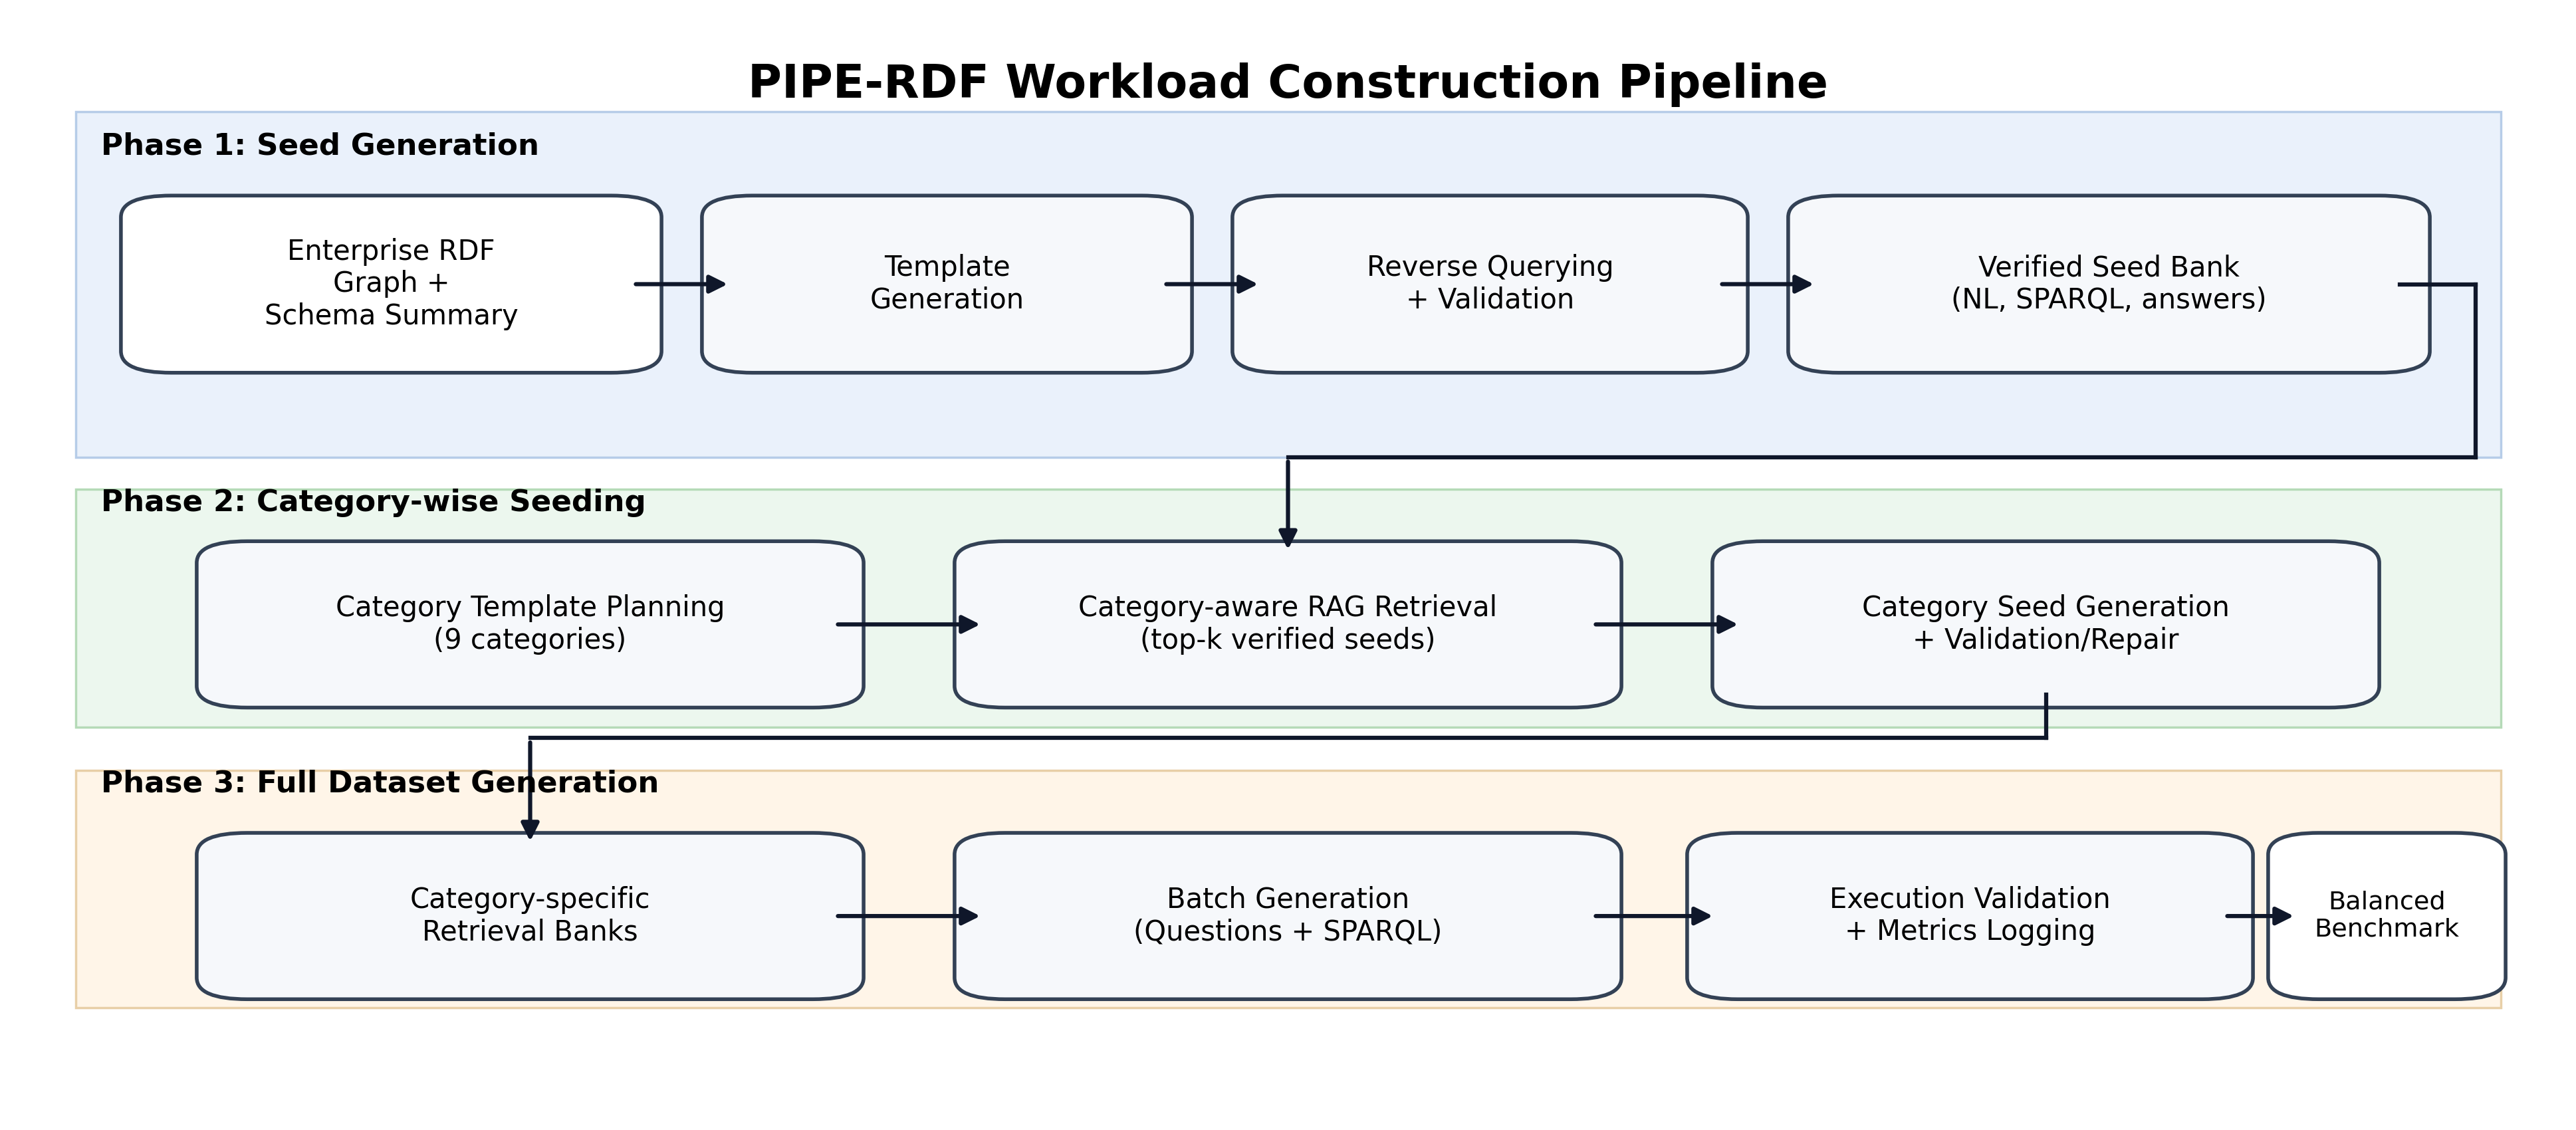
\includegraphics[width=0.95\linewidth]{figures/pipeline_architecture.png}
  \caption{PIPE-RDF workload-construction pipeline: Phase 1 uses reverse query generation to build verified seeds; Phase 2 constructs category-specific seed banks; Phase 3 generates the balanced benchmark with execution-driven validation/repair.}
  \label{fig:pipeline}
\end{figure}

\section{Schemas and Implementation}
\textbf{Fixed schema slice.} We derive a company-location mini-slice (Schema C) with 5{,}000 companies and three classes: \texttt{dbo:Company}, \texttt{gn:Feature} (location), and \texttt{foaf:Person} (key person), illustrated in Appendix Figure~\ref{fig:app_schema_ontology}. The allowed predicates are \texttt{dbo:location}, \texttt{dbo:industry}, \texttt{dbo:keyPerson}, \texttt{dbo:foundingYear}, \texttt{dbo:numberOfEmployees}, and label predicates (\texttt{rdfs:label}, \texttt{spb:prefLabel}, \texttt{foaf:name}). This fixed schema avoids prompt drift and simplifies validation.

\textbf{Slice extraction.} The mini-slice is sampled from a public RDF source by selecting companies with at least one of the core predicates (location, industry, key person, founding year, or employee count). Linked entities (locations and key people) are included with minimal labels to support question instantiation without introducing extraneous schema elements. We intentionally exclude unrelated predicates to reduce template drift and ensure that reverse querying remains tractable.

\textbf{SPB-full schema.} To test the same method beyond the compact slice, we also run on a full LDBC Semantic Publishing Benchmark graph with roughly 25M triples. The graph contains many more entity types and predicates than Schema C; its top predicates include \texttt{rdf:type}, \texttt{spb:prefLabel}, \texttt{foaf:name}, \texttt{dbo:birthPlace}, \texttt{dbo:location}, \texttt{dbo:foundingYear}, \texttt{dbo:industry}, \texttt{dbo:keyPerson}, and \texttt{dbo:numberOfEmployees}. For comparability, the benchmark-generation task still targets the company/location/person-style query categories, while the schema summary and whitelist are derived from the larger graph. This separates graph scale and schema-profile breadth from changes in task taxonomy.

\begin{table}[t]
  \centering
  \small
  \setlength{\tabcolsep}{4pt}
  \begin{tabularx}{\linewidth}{>{\raggedright\arraybackslash}p{0.26\linewidth} X}
    \toprule
    Class & Key predicates/attributes \\
    \midrule
    \texttt{dbo:Company} & \texttt{dbo:location}, \texttt{dbo:industry}, \texttt{dbo:keyPerson}, \\
    & \texttt{dbo:foundingYear}, \texttt{dbo:numberOfEmployees}, \texttt{rdfs:label} \\
    \texttt{gn:Feature} & \texttt{rdfs:label}, \texttt{spb:prefLabel} \\
    \texttt{foaf:Person} & \texttt{foaf:name}, \texttt{rdfs:label} \\
    \bottomrule
  \end{tabularx}
  \caption{Schema C mini-slice classes and allowed predicates.}
  \label{tab:schema}
\end{table}

\textbf{Pipeline configuration.} The original baseline used 5 templates per category with 8 seed instantiations per template in Phase 1, 20 seeds per category in Phase 2, and 50 targets per category in Phase 3. The expanded runs increase Phase 3 to 200 targets per category on each of two schemas (3{,}600 Phase-3 pairs total). Generated SPARQL is capped at 5 results to limit execution cost. Binding banks use bounded deterministic pools and client-side shuffling for diversity.

\begin{table}[t]
  \centering
  \small
  \resizebox{\linewidth}{!}{
  \begin{tabular}{ll}
    \toprule
    Parameter & Value \\
    \midrule
    Phase 1 templates / category & 5 \\
    Phase 1 seeds / template & 8 \\
    Phase 2 seeds / category & 20 \\
    Phase 3 targets / category & 50 baseline / 200 expanded \\
    Binding-bank pool & bounded deterministic pool \\
    Retrieval top-$k$ & 2 \\
    SPARQL result cap & 5 \\
    Dedup Jaccard threshold & 0.99 \\
    \bottomrule
  \end{tabular}
  }
\caption{Key pipeline configuration. The expanded runs keep the same category taxonomy while scaling Phase 3 targets and moving reverse-query work into deterministic binding-bank construction.}
  \label{tab:config}
\end{table}

\textbf{Runtime environment.} We run GraphDB 10.6.3 and execute SPARQL with inference disabled. The expanded generation uses Qwen 3.5 models served through vLLM and local \texttt{BAAI/bge-m3} embeddings. The primary runs use \texttt{Qwen/Qwen3.5-4B}; robustness probes use \texttt{Qwen/Qwen3.5-2B}, \texttt{Qwen/Qwen3.5-4B}, and \texttt{Qwen/Qwen3.5-9B}. All runs are logged with execution latency, parse validity, and answer counts; artifacts are exported as JSONL/CSV and summarized in run-level reports. A compact reproducibility checklist is provided in Appendix Section~\ref{app:repro}.

\textbf{SPARQL formalism and schema constraints.} To ensure semantic correctness, we enforce canonical query patterns:
\begin{itemize}
  \item \textbf{Counting}: Use \texttt{COUNT(DISTINCT ?var)} to avoid overcounting due to multiple bindings.
  \item \textbf{Superlative/Ordinal}: Include deterministic tie-breaking via \texttt{ORDER BY ... ?entity} to ensure reproducible results.
  \item \textbf{Numeric comparisons}: Cast literals to \texttt{xsd:integer} where applicable (e.g., \texttt{dbo:numberOfEmployees}).
  \item \textbf{Yes/No}: Use \texttt{ASK \{\}} for explicit boolean returns, avoiding empty-result ambiguity.
\end{itemize}
Schema constraints are enforced via predicate whitelists: \texttt{dbo:location} ranges over \texttt{gn:Feature}, \texttt{dbo:keyPerson} ranges over \texttt{foaf:Person}, and \texttt{dbo:foundingYear}/\texttt{dbo:numberOfEmployees} are typed literals. Label resolution prioritizes \texttt{foaf:name} for persons, \texttt{rdfs:label} for companies, and \texttt{spb:prefLabel} for locations.

\section{Evaluation Protocol}
PIPE-RDF logs operational and structural metrics for every generated pair. We track: (i) parse validity and execution success, (ii) non-empty answer coverage, (iii) repair attempts, (iv) answer counts, (v) prompt and question lengths, (vi) LLM latency, and (vii) SPARQL structural complexity (triple pattern counts, FILTER clauses, aggregations). These metrics support both data quality analysis and model evaluation. While PIPE-RDF focuses on execution-driven correctness, the artifacts can be augmented with SPARQL-specific metrics (SP-F1) and structural metrics (CodeBLEU) for model evaluation \citep{Rony_2022,ren2020codebleumethodautomaticevaluation}. We also record retrieval scores to analyze the relationship between example similarity and downstream execution success.

Following recent workload-generation evaluation practice \citep{agarwal2024crossmodel}, we additionally report strategy coverage and strategy-level error breakdowns to make pipeline behavior auditable beyond aggregate success rates. Strategy tags are inferred from query operators (JOIN, FILTER, COUNT, ORDER, NEGATION, ASK, RAG-context). ASK and NEGATION tags are retained in coverage/error matrices even when observed frequency is zero in Phase 3 outputs.

\textbf{Semantic correctness audit.} To verify that generated NL--SPARQL pairs are semantically aligned (not just syntactically valid), we construct a 216-pair stratified audit packet: 2 schemas \(\times\) 9 categories \(\times\) 12 pairs. Two annotators independently check whether (i) question intent matches the SPARQL semantics, (ii) entity bindings in the question correspond to VALUES clauses or equivalent query constraints, (iii) the answer type matches the expected return, and (iv) the category label matches the dominant SPARQL construct. The accompanying agreement script reports pass rate, Cohen's \(\kappa\), disagreement counts, and adjudicated error categories once annotation files are completed.

\section{Benchmark Results}
The primary expanded evaluation uses \texttt{Qwen/Qwen3.5-4B} served through vLLM. We generate 1{,}800 Phase-3 pairs for each schema, with exactly 200 pairs in each of the nine categories. Table~\ref{tab:arr_schema_scale} summarizes the strict final-artifact checks. A record is accepted only if its SPARQL parses, executes, returns a category-appropriate answer object, avoids zero-count counting artifacts, and passes category-form checks such as \texttt{COUNT} for counting and ranked \texttt{ORDER BY}/\texttt{OFFSET} forms for ordinal queries. Both schemas satisfy these checks without repair calls.

\begin{table}[t]
  \centering
  \small
  \resizebox{\linewidth}{!}{
  \begin{tabular}{lrrrrrrr}
    \toprule
    Schema & Graph scale & Pairs & Min/Max cat. & Parse fail & Exec fail & Empty & Repairs \\
    \midrule
    Schema C & 38K triples, 3 types & 1{,}800 & 200/200 & 0 & 0 & 0 & 0 \\
    SPB-full & 25M triples, broad type/predicate profile & 1{,}800 & 200/200 & 0 & 0 & 0 & 0 \\
    \bottomrule
  \end{tabular}
  }
  \caption{Primary expanded Phase-3 results. Both schemas are balanced at 200 examples per category across nine categories and pass strict parse, execution, answer-type, and category-form checks.}
  \label{tab:arr_schema_scale}
\end{table}

\begin{table}[t]
  \centering
  \small
  \resizebox{\linewidth}{!}{
  \begin{tabular}{lrrrrrr}
    \toprule
    Schema & LLM ms & SPARQL ms & Question ms & Predicates used & Zero-count & ASK type err. \\
    \midrule
    Schema C & 650.5 & 3.7 & 0.05 & 6 & 0 & 0 \\
    SPB-full & 1596.0 & 5.6 & 0.06 & 8 & 0 & 0 \\
    \bottomrule
  \end{tabular}
  }
  \caption{Runtime and strict answer-shape diagnostics for the two primary runs. LLM time dominates end-to-end generation; SPARQL execution remains in the single-digit millisecond range after binding-bank construction and batched metadata lookup.}
  \label{tab:primary_runtime}
\end{table}

\section{Cross-Model Robustness}
\label{sec:arr_scale}
To test whether the pipeline depends on a single LLM size, we rerun 50-pair-per-category probes with Qwen3.5-2B, Qwen3.5-4B, and Qwen3.5-9B on both schemas. These probes use the same strict acceptance checks as the primary runs. Table~\ref{tab:qwen35_robustness} shows that all six probes are balanced and produce 100\% parse and execution validity with no empty answers and no repairs. This does not imply that every intermediate LLM proposal is correct; rather, it shows that reverse-query grounding plus strict validation produces reliable accepted artifacts across smaller and larger open models.

\begin{table}[t]
  \centering
  \small
  \resizebox{\linewidth}{!}{
  \begin{tabular}{llrrrrr}
    \toprule
    Schema & Model & Pairs & Parse fail & Exec fail & Empty & SPARQL ms \\
    \midrule
    Schema C & Qwen3.5-2B & 450 & 0 & 0 & 0 & 4.1 \\
    Schema C & Qwen3.5-4B & 450 & 0 & 0 & 0 & 16.7 \\
    Schema C & Qwen3.5-9B & 450 & 0 & 0 & 0 & 5.0 \\
    SPB-full & Qwen3.5-2B & 450 & 0 & 0 & 0 & 8.2 \\
    SPB-full & Qwen3.5-4B & 450 & 0 & 0 & 0 & 5.8 \\
    SPB-full & Qwen3.5-9B & 450 & 0 & 0 & 0 & 7.2 \\
    \bottomrule
  \end{tabular}
  }
  \caption{Cross-model generation robustness probes at 50 pairs per category per schema.}
  \label{tab:qwen35_robustness}
\end{table}

\section{Semantic Audit and Benchmark Utility}
\label{sec:audit_utility}
The semantic audit addresses the gap between executable queries and semantically correct NL--SPARQL pairs. We prepared a 216-pair audit packet sampled uniformly by schema and category: 2 schemas \(\times\) 9 categories \(\times\) 12 pairs. The packet includes the question, SPARQL, normalized answer, category, schema, and annotation fields for intent/query match, entity-binding correctness, answer-type correctness, category correctness, pass/fail, and error type. We also provide an agreement script that computes exact agreement and Cohen's \(\kappa\) over the shared pair identifiers.

\begin{table}[t]
  \centering
  \small
  \resizebox{\linewidth}{!}{
  \begin{tabular}{lrrrr}
    \toprule
    Schema & Packet size & Categories & Per cat. & Status \\
    \midrule
    Schema C & 108 & 9 & 12 & prepared for annotation \\
    SPB-full & 108 & 9 & 12 & prepared for annotation \\
    \bottomrule
  \end{tabular}
  }
  \caption{Semantic audit packet prepared for independent two-annotator review. Quantitative pass rate, agreement, \(\kappa\), and adjudicated errors require completed annotation files.}
  \label{tab:semantic_audit}
\end{table}

We also evaluate whether the generated benchmark is useful for NL-to-SPARQL prompting. On 180 held-out pairs per condition, we compare a schema-only zero-shot prompt against category-retrieval prompts using \(k=3\) generated examples. Table~\ref{tab:downstream_utility} shows large and consistent improvements from category retrieval. For Qwen3.5-2B, category-RAG raises answer F1 from 1.7 to 86.1 on Schema C and from 5.6 to 89.2 on SPB-full. For Qwen3.5-4B, category-RAG raises answer F1 from 32.8 to 91.1 on Schema C and from 18.3 to 90.0 on SPB-full. These results support the benchmark's practical utility as a source of schema- and category-matched examples, not only as a static evaluation set.

\begin{table}[t]
  \centering
  \small
  \resizebox{\linewidth}{!}{
  \begin{tabular}{lllrrrr}
    \toprule
    Schema & Model & Setting & Parse\% & Exec\% & Answer F1 & SP-F1 \\
    \midrule
    Schema C & Qwen3.5-2B & Zero-shot & 45.0 & 45.0 & 1.7 & 82.5 \\
    Schema C & Qwen3.5-2B & Category-RAG & 100.0 & 100.0 & 86.1 & 99.7 \\
    Schema C & Qwen3.5-4B & Zero-shot & 75.0 & 73.3 & 32.8 & 89.9 \\
    Schema C & Qwen3.5-4B & Category-RAG & 99.4 & 99.4 & 91.1 & 99.7 \\
    SPB-full & Qwen3.5-2B & Zero-shot & 38.3 & 35.6 & 5.6 & 72.0 \\
    SPB-full & Qwen3.5-2B & Category-RAG & 100.0 & 100.0 & 89.2 & 99.8 \\
    SPB-full & Qwen3.5-4B & Zero-shot & 84.4 & 84.4 & 18.3 & 83.2 \\
    SPB-full & Qwen3.5-4B & Category-RAG & 100.0 & 100.0 & 90.0 & 99.7 \\
    \bottomrule
  \end{tabular}
  }
  \caption{Downstream utility evaluation on 180 held-out examples per schema/model/setting. Category-RAG uses \(k=3\) generated examples from the same schema and target category.}
  \label{tab:downstream_utility}
\end{table}

\section{Discussion and Operational Lessons}
The reviewer concerns motivating this revision were scale, generality beyond one compact schema, LLM dependence, and semantic validation. The new results directly address the first three: the primary benchmark grows from 450 to 3{,}600 Phase-3 pairs; the second schema uses a much larger public RDF graph; and cross-model probes show that strict accepted artifacts are not tied to one Qwen 3.5 model size. The downstream utility experiment adds a separate usefulness claim: generated category-matched examples materially improve held-out NL-to-SPARQL prompting, especially for smaller models.

The most important operational lesson is that SPARQL endpoint design matters as much as model choice when scaling benchmark generation. The initial large-graph runs exposed endpoint bottlenecks from randomized reverse queries and many tiny metadata lookups. Replacing \texttt{ORDER BY RAND()} with deterministic binding banks, shuffling locally, and batching label/type retrieval reduced GraphDB load enough to complete balanced 200-per-category runs. This supports the pipeline's methodological claim: execution grounding is practical when reverse-query work is treated as a planned data-building stage rather than an online sampling side effect.

The remaining semantic-audit step is intentionally separated from automated validity. Parse and execution validity prove that queries are legal and answerable; they do not prove that the natural-language question perfectly matches the SPARQL intent. The audit packet and agreement tooling make this check reproducible, but the final pass rate and \(\kappa\) should be reported only after independent annotations are completed.

\section{Benchmark Usage}
\label{sec:benchmark_usage}
PIPE-RDF produces benchmark artifacts that can be used to evaluate NL-to-SPARQL systems on a target RDF schema. The generated pairs support execution accuracy, answer F1, SP-F1, and structural similarity evaluation. The same seed banks can also be reused as few-shot retrieval examples or synthetic supervision for schema-specific fine-tuning. The method is especially useful when public KGQA datasets do not match the target ontology, but the contribution does not depend on demonstrating adoption in any particular deployment context.

\section{Conclusion}
\label{sec:conclusion}
PIPE-RDF provides a practical pipeline for generating balanced, schema-specific NL--SPARQL benchmarks. Across two RDF schemas, the primary Qwen3.5-4B runs produce 3{,}600 strictly valid Phase-3 pairs with exact category balance, no parse failures, no execution failures, no empty answers, and no repairs. Cross-model probes with Qwen3.5-2B, 4B, and 9B show the same strict accepted-artifact profile at smaller scale, and the downstream utility evaluation shows that generated category-matched examples substantially improve NL-to-SPARQL prompting. By combining reverse querying, category-aware retrieval, binding banks, and execution-based validation, PIPE-RDF supports reproducible benchmark construction for RDF question answering.

\section{Limitations}
\label{sec:limitations}
Both evaluated schemas are public. Schema C is a controlled public company-location slice and SPB-full is a public benchmark graph; we do not claim evidence from private or proprietary deployments. This is a deliberate change from an industry-track framing: the paper's claim is about schema-specific benchmark construction, not about the prevalence or adoption of RDF/SPARQL in any particular sector.

The semantic audit is prepared but requires independent human annotation before the paper should report pass rates and Cohen's \(\kappa\). Automated parse, execution, and answer-shape checks are necessary quality gates, but they are not substitutes for semantic alignment judgments.

The downstream utility evaluation is prompt-based rather than a full comparison of fine-tuned semantic parsers. It shows that generated examples improve retrieval-augmented prompting, but future work should evaluate fine-tuning, grammar-constrained decoding, and additional RDF schemas with different ontology styles. The Qwen3.5-9B probe required a shorter 8K context on one GPU because the 16K configuration exceeded available memory; all probe prompts fit within that context, but larger-context deployments should report serving constraints explicitly.

\section{Ethical Considerations}
\label{sec:ethical}
PIPE-RDF is intended for benchmark construction over RDF graphs. When used with private graphs, deployments should follow data governance policies, minimize exposure of sensitive identifiers in prompts, and audit logs for leakage. The public schemas in this study are derived from public RDF data, and usage follows their licensing terms.

\bibliography{references}

\appendix
\section*{Appendix}
\section{Extended Operational Analysis}
\label{app:extended_analysis}

This appendix reports detailed diagnostics that were omitted from the main paper for ACL page-budget constraints. The key interpretation in all plots and tables is unchanged from the main text: pipeline reliability is high, and most residual difficulty is due to sparse conjunctive semantics rather than parser instability.

\subsection{Reproducibility Checklist}
\label{app:repro}
\begin{itemize}
  \item \textbf{Software/models}: GraphDB 10.6.3 (Docker), vLLM service, Qwen 3.5 chat models, embedding model \texttt{BAAI/bge-m3}.
  \item \textbf{Endpoint/repository}: repository \emph{spb\_company\_mini\_slice} with inference disabled (\texttt{infer=false}); see run log for full endpoint string.
  \item \textbf{Configuration}: main run uses the full-run YAML config; key sizes are listed in Table~\ref{tab:config}.
  \item \textbf{Randomness control}: seed control is exposed via \texttt{SEED=42} in \texttt{pipekg/config.py}. LLM generation remains stochastic; we therefore release full run artifacts for exact reuse of produced pairs.
  \item \textbf{Command template}: \texttt{python scripts/run\_pipeline\_ollama.py} with expanded-run configs under \texttt{configs/arr\_*.yaml}.
  \item \textbf{Artifacts}: \texttt{run.log}, \texttt{pipeline\_records.jsonl}, phase-wise JSONL/CSV, analysis summaries, and figures under \texttt{artifacts/runs/<run\_id>/}.
  \item \textbf{Hardware/deployment}: GraphDB in Docker plus vLLM model serving on GPU resources; per-query latencies are reported in the main paper.
\end{itemize}

\textbf{Category and strategy diagnostics.} Figure~\ref{fig:category_radar} highlights structural differences across categories, and Appendix Figure~\ref{fig:strategy_error_appendix} reports strategy-conditioned error rates. These legacy diagnostics come from the earlier 450-pair baseline artifact; the expanded strict artifacts supersede their validity and empty-answer statistics, but the plots remain useful for illustrating the diagnostic reports produced by the pipeline.

\begin{figure}[h]
  \centering
  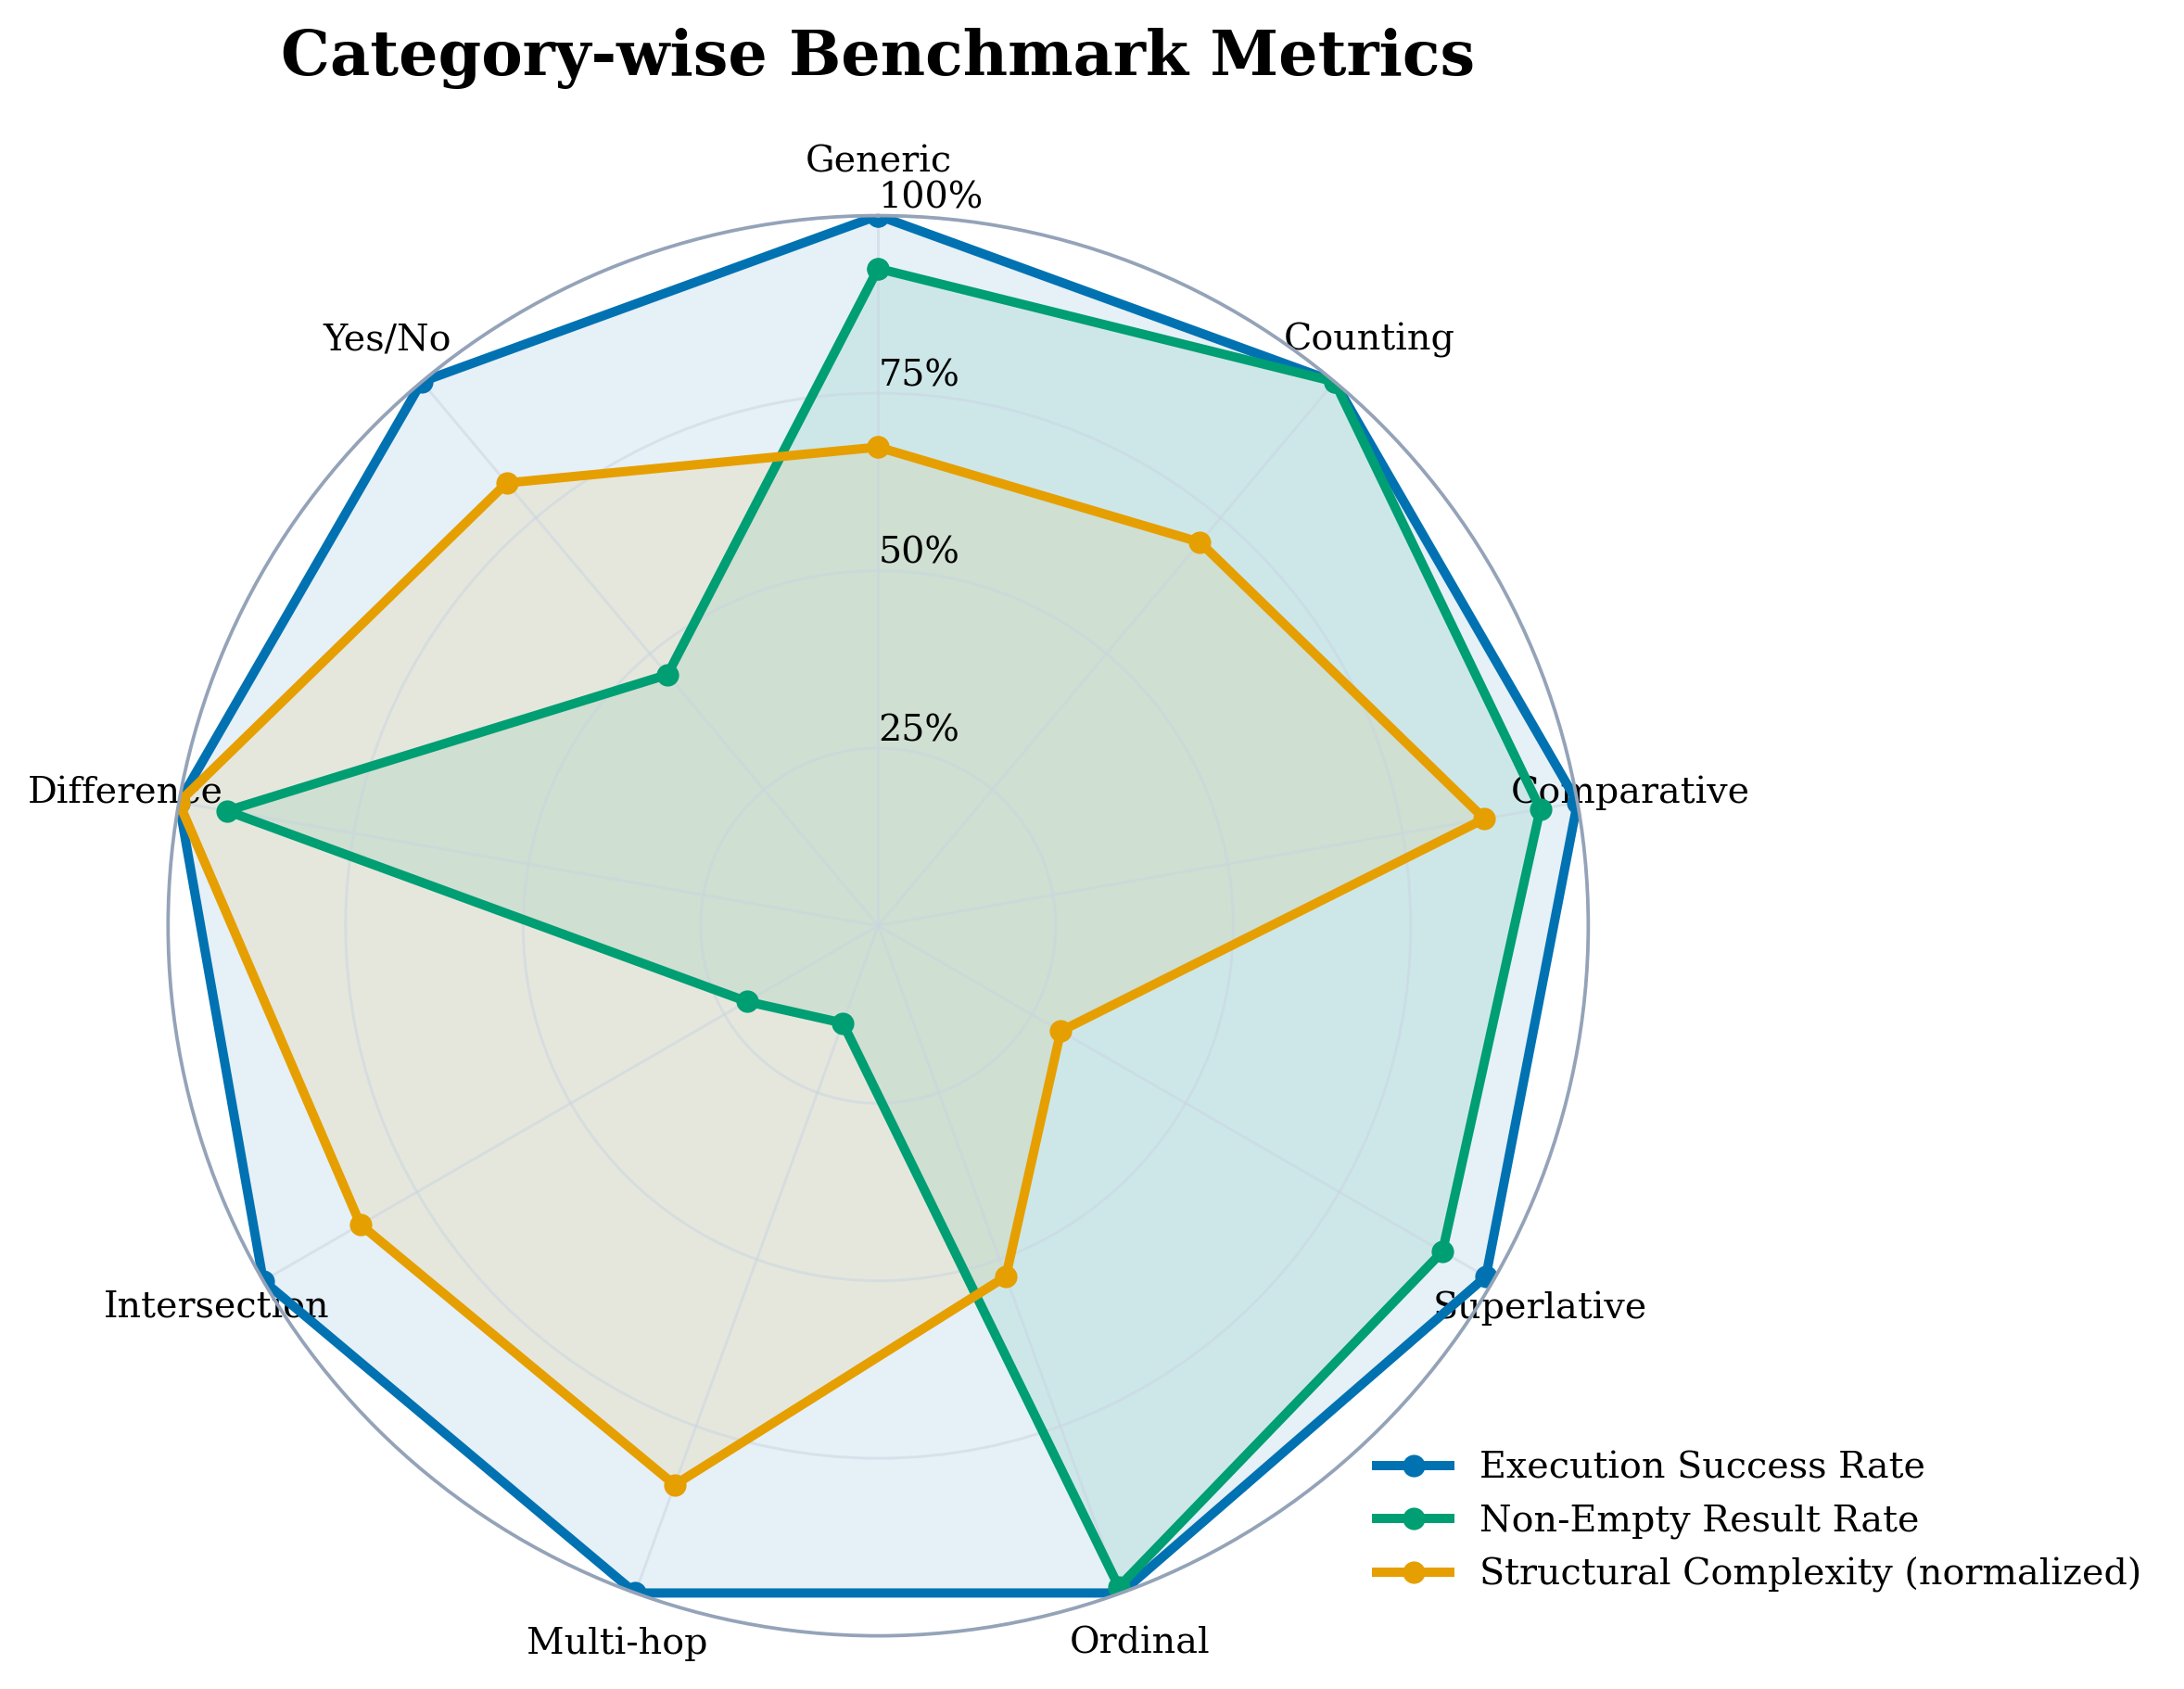
\includegraphics[width=0.95\linewidth]{figures/category_radar.png}
  \caption{Category-wise metrics: execution success (100\%), non-empty rate, and normalized structural complexity.}
  \label{fig:category_radar}
\end{figure}

\begin{figure}[h]
  \centering
  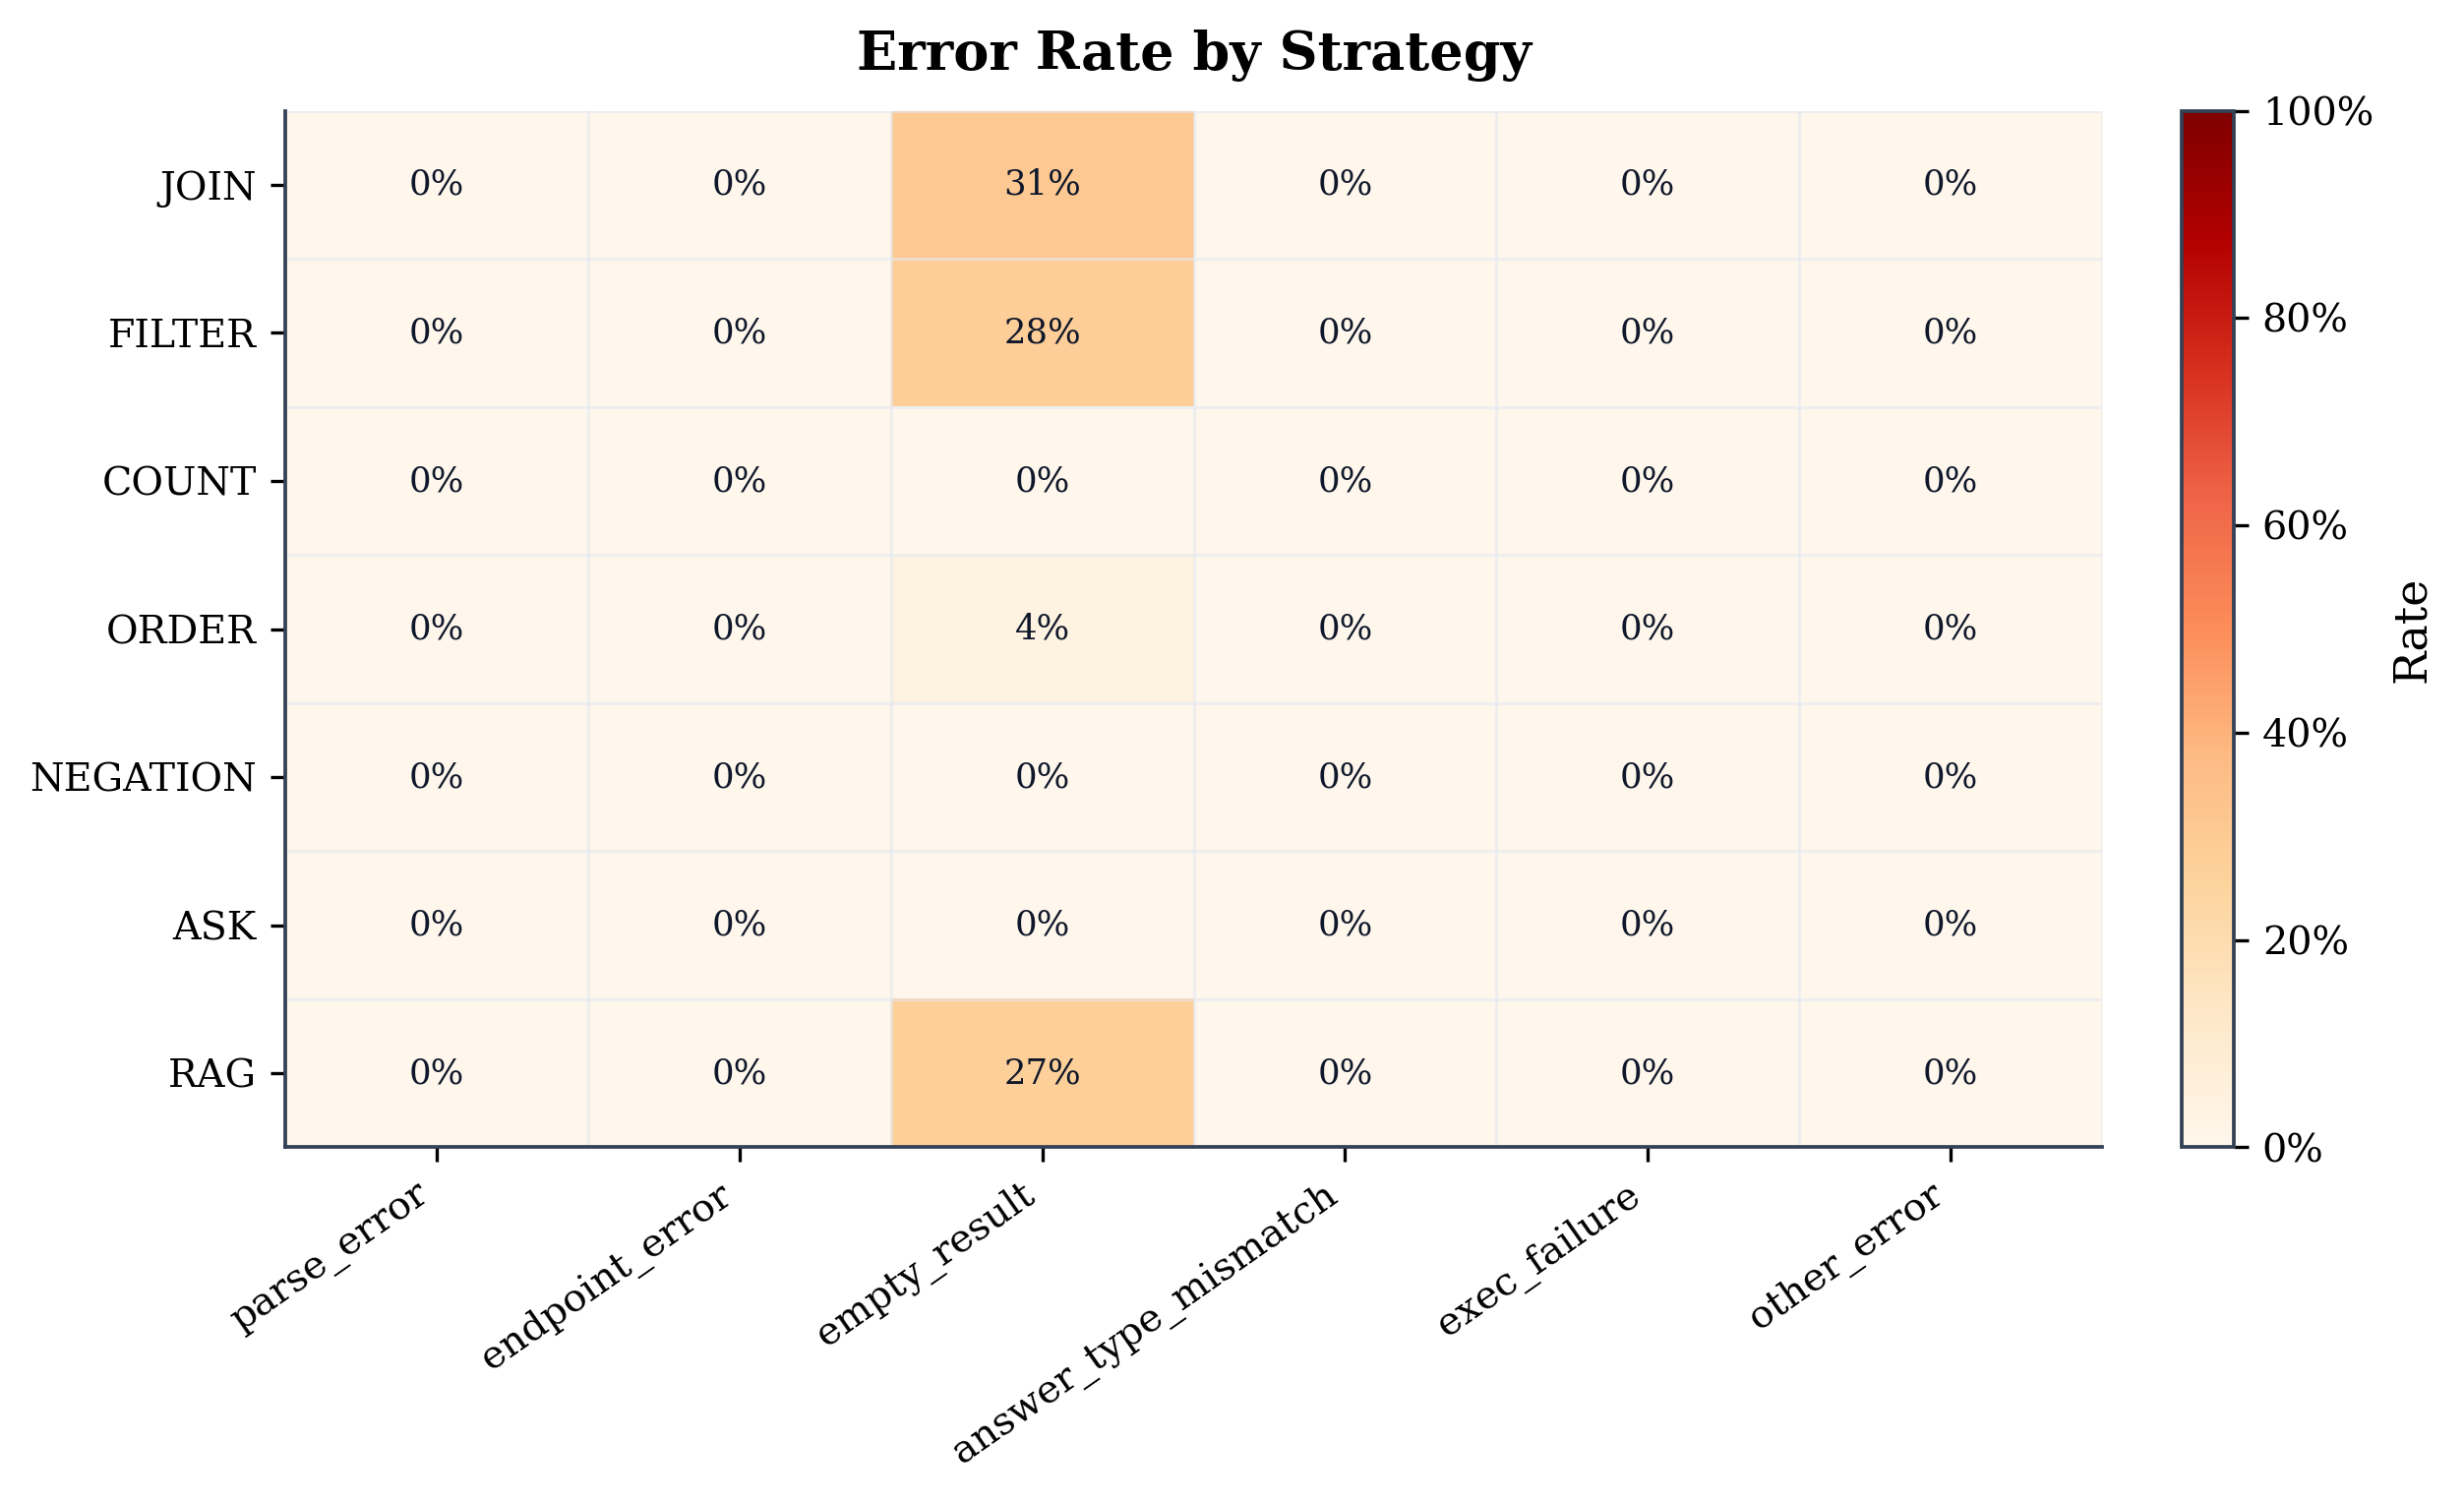
\includegraphics[width=0.95\linewidth]{figures/strategy_error_heatmap_phase3.png}
  \caption{Phase 3 strategy-conditioned error rates. Non-zero cells are concentrated in empty-result outcomes for sparse conjunctive structures.}
  \label{fig:strategy_error_appendix}
\end{figure}

\textbf{Data quality controls and throughput.} In error analysis, we observed a small number of self-comparison pairs, retrieval self-reference cases, and answer-type mismatches; we implemented automated guards for each. Runtime remains generation-bound: average LLM latency is 5.3s per query versus about 7ms SPARQL latency. These measurements support production prioritization toward prompt and inference optimization rather than query engine tuning.

\section{Additional Figures}
\label{app:figures}

\begin{figure}[h]
  \centering
  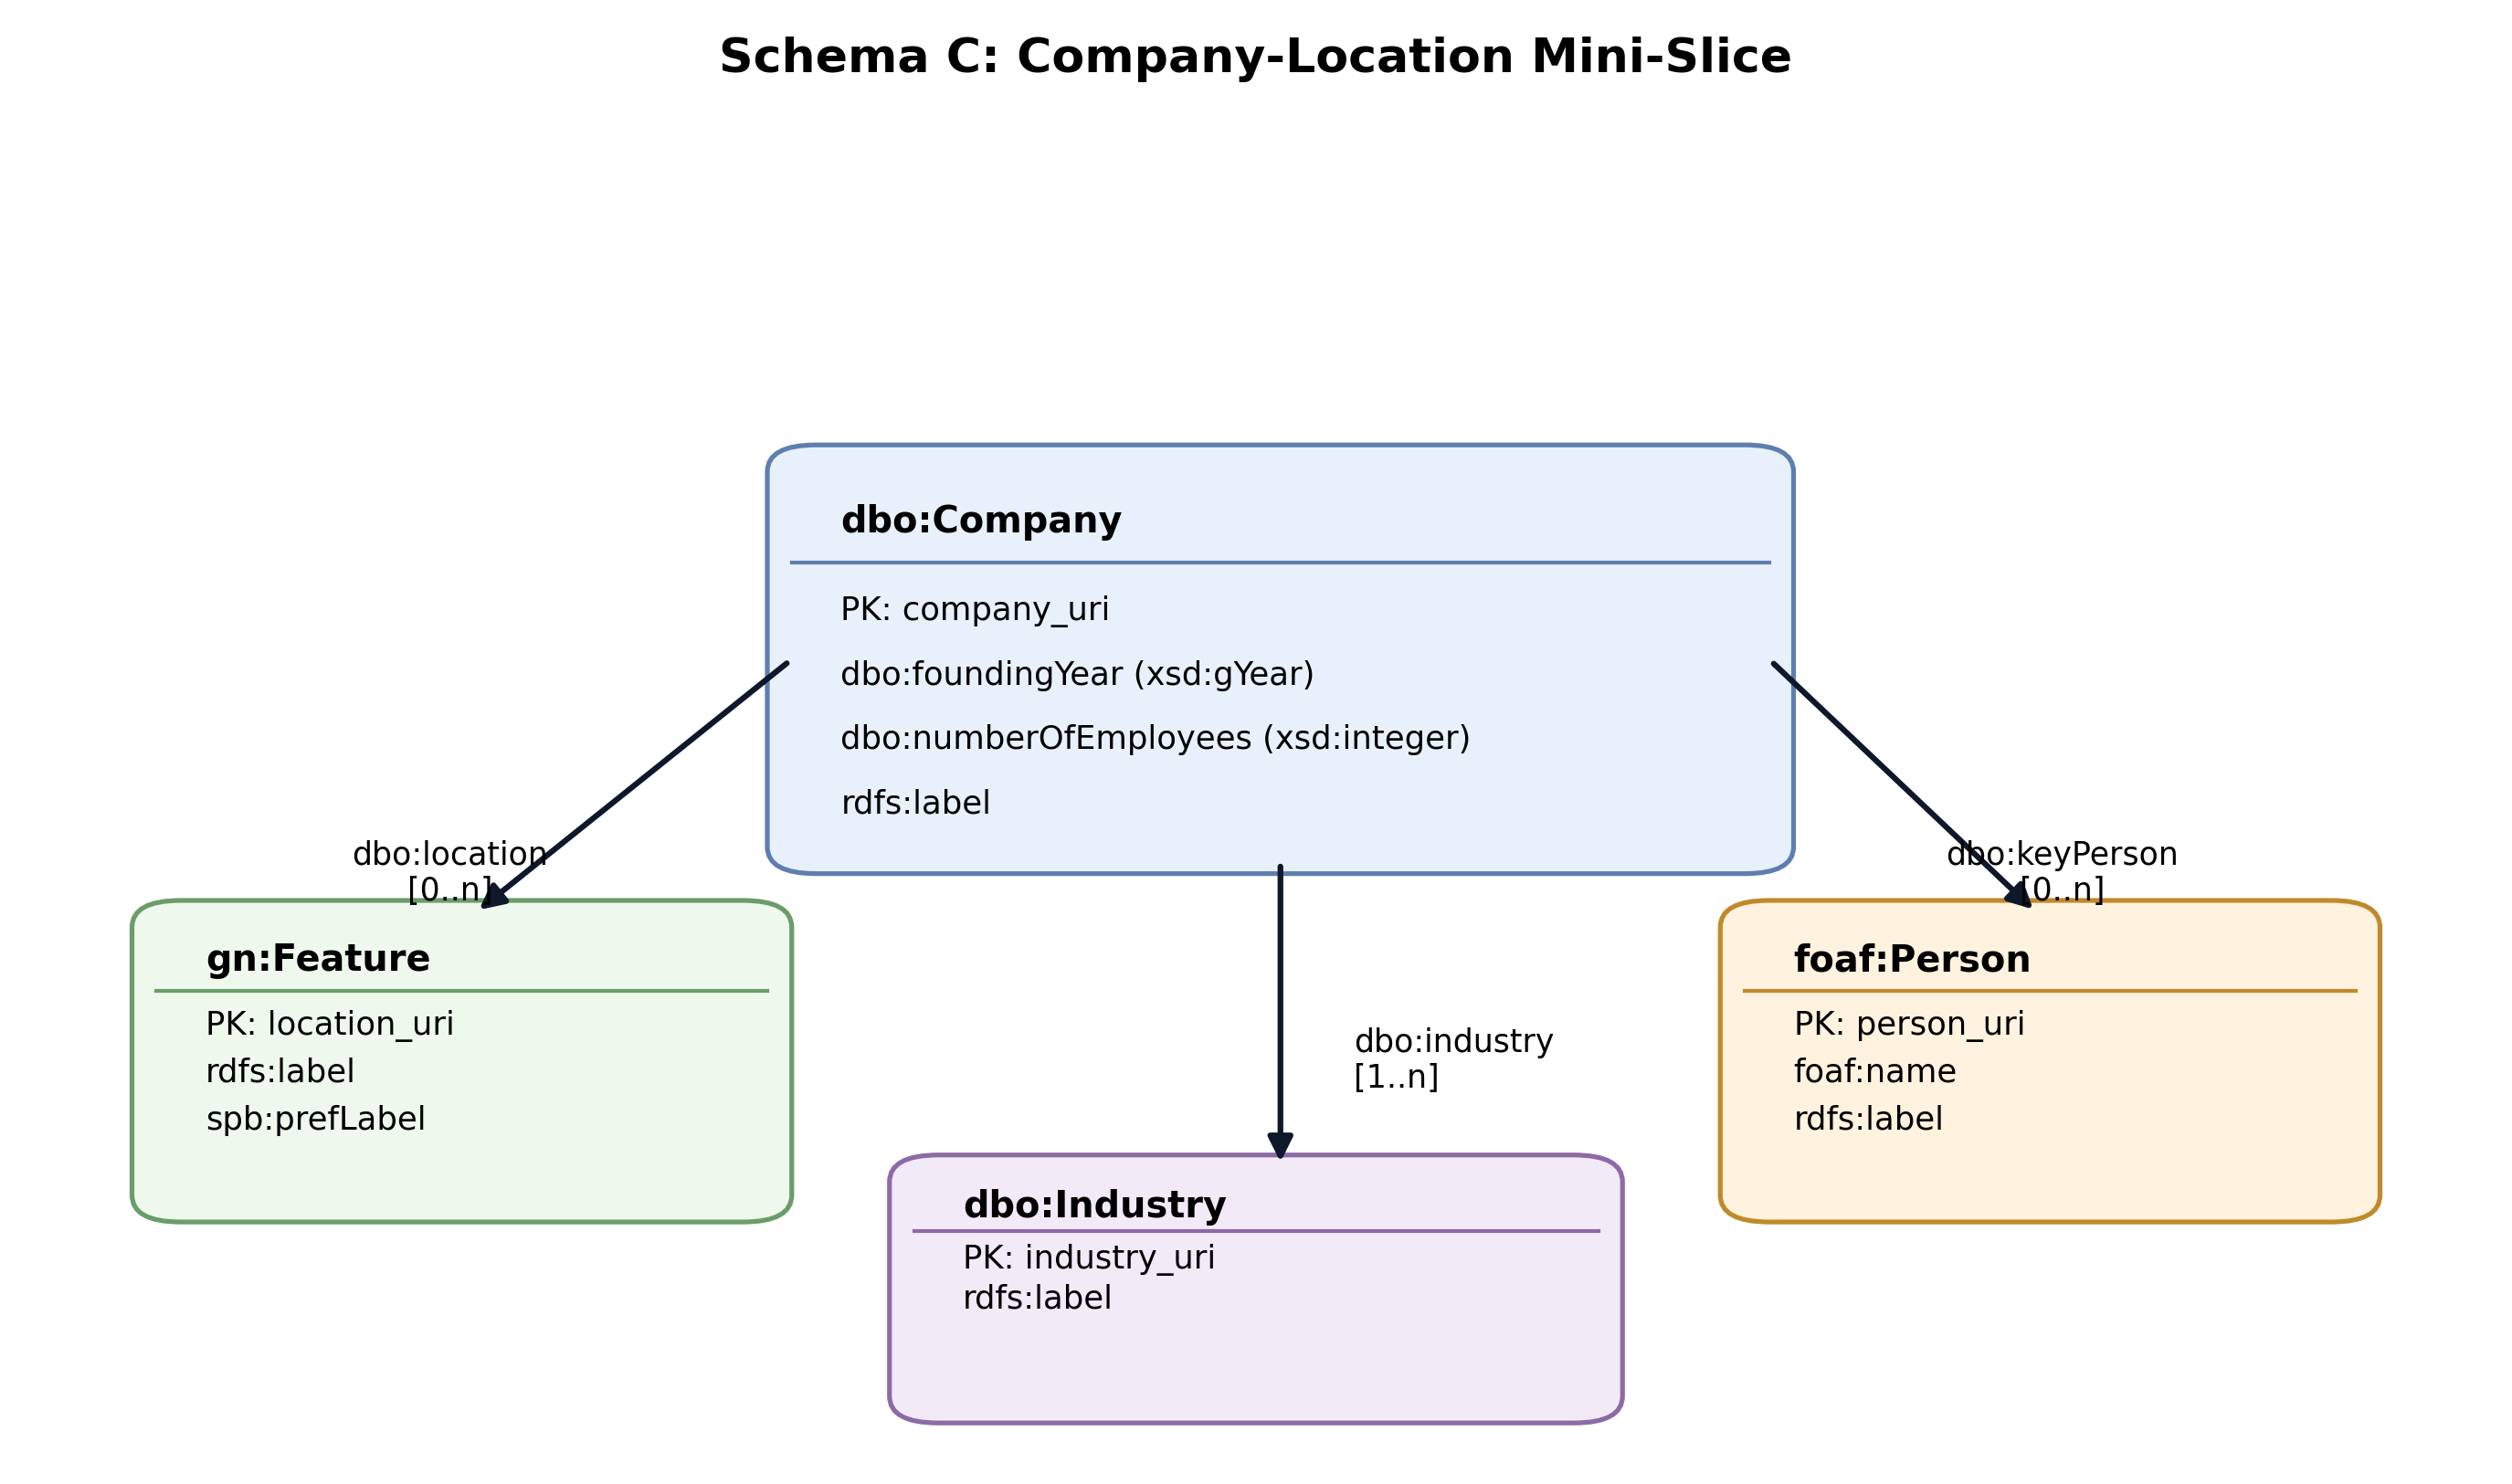
\includegraphics[width=0.95\linewidth]{figures/schema_ontology.png}
  \caption{Schema C ontology used in this study. \texttt{dbo:Company} connects to \texttt{gn:Feature} (location), \texttt{foaf:Person} (key person), and \texttt{dbo:Industry} with typed predicates and cardinalities.}
  \label{fig:app_schema_ontology}
\end{figure}

\begin{figure}[h]
  \centering
  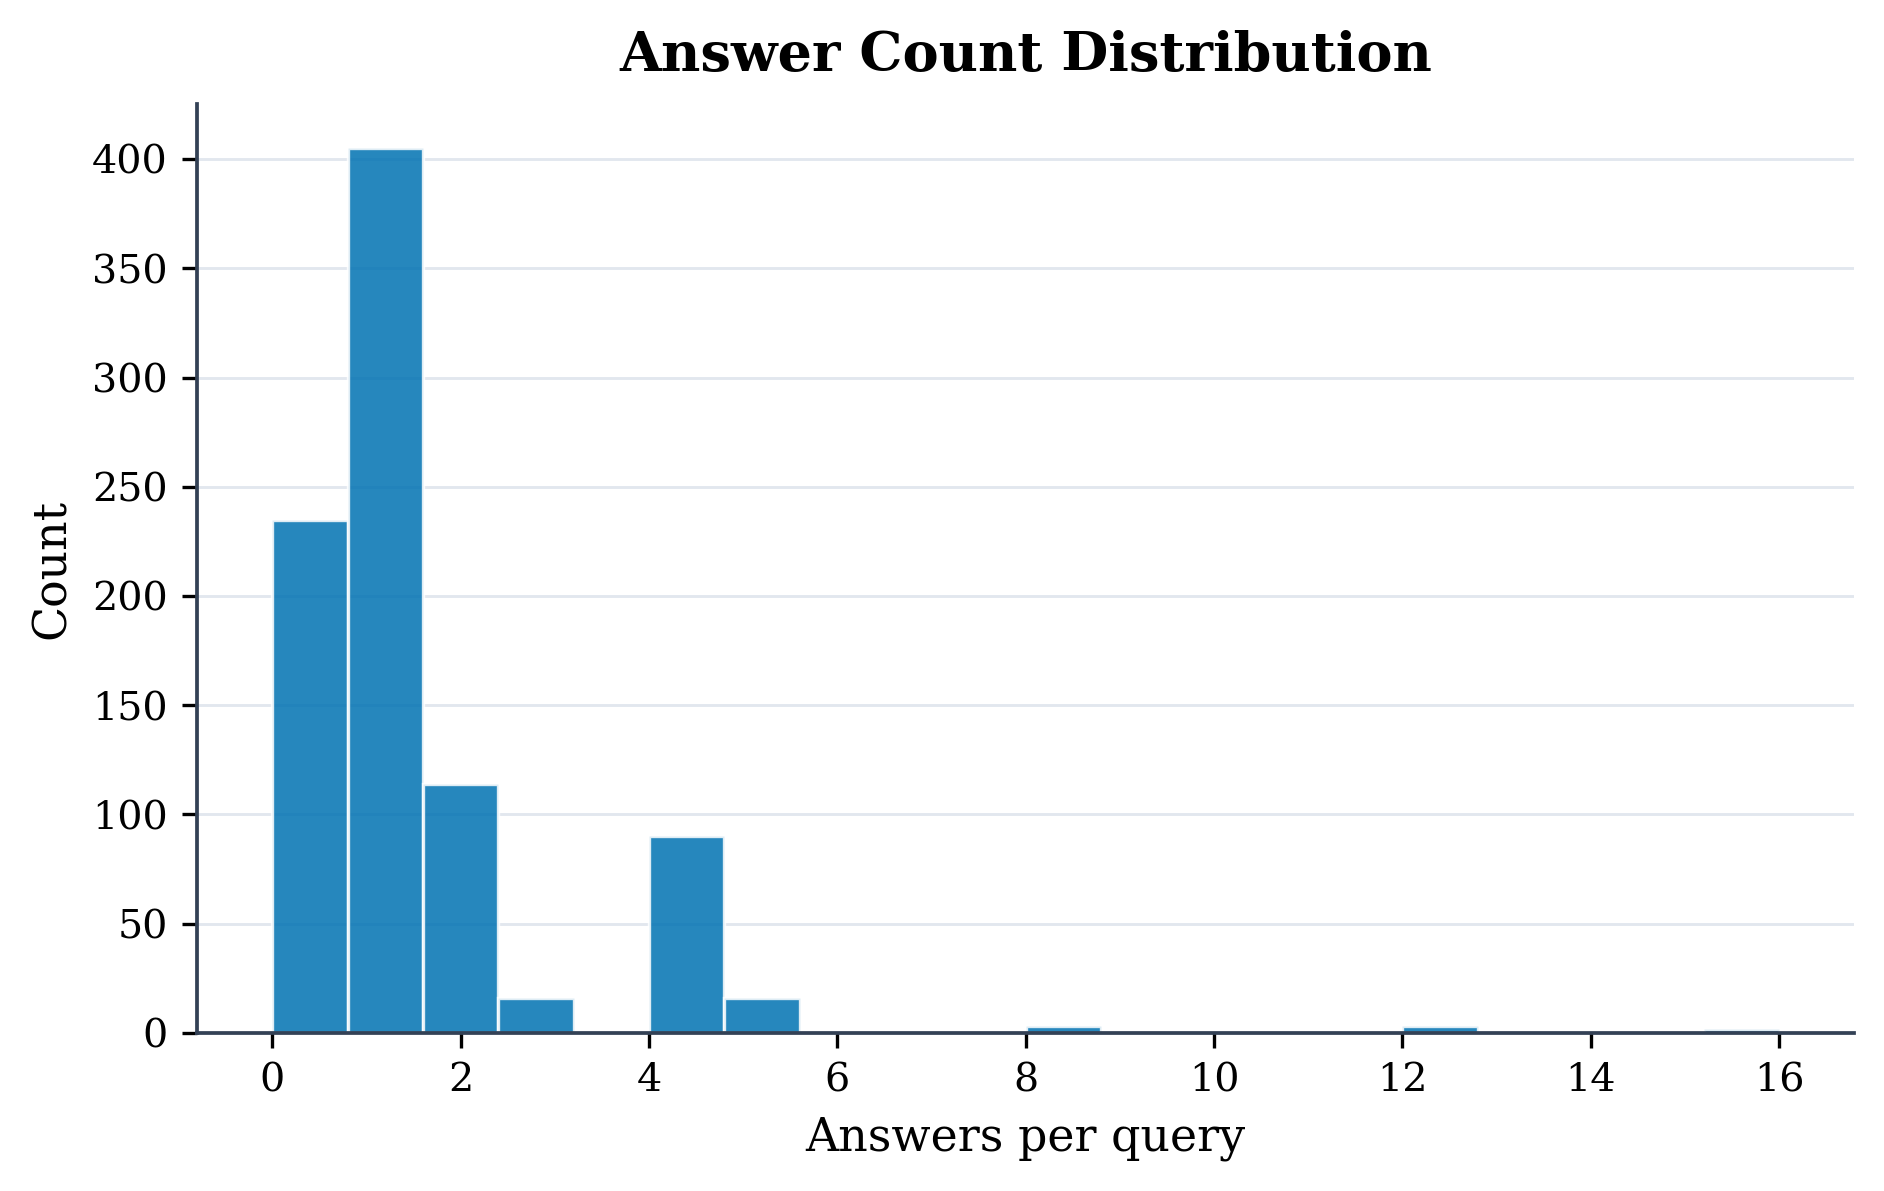
\includegraphics[width=0.95\linewidth]{figures/answer_count_hist.png}
  \caption{Answer count distribution for Phase 3.}
  \label{fig:answer_counts}
\end{figure}

\begin{figure}[h]
  \centering
  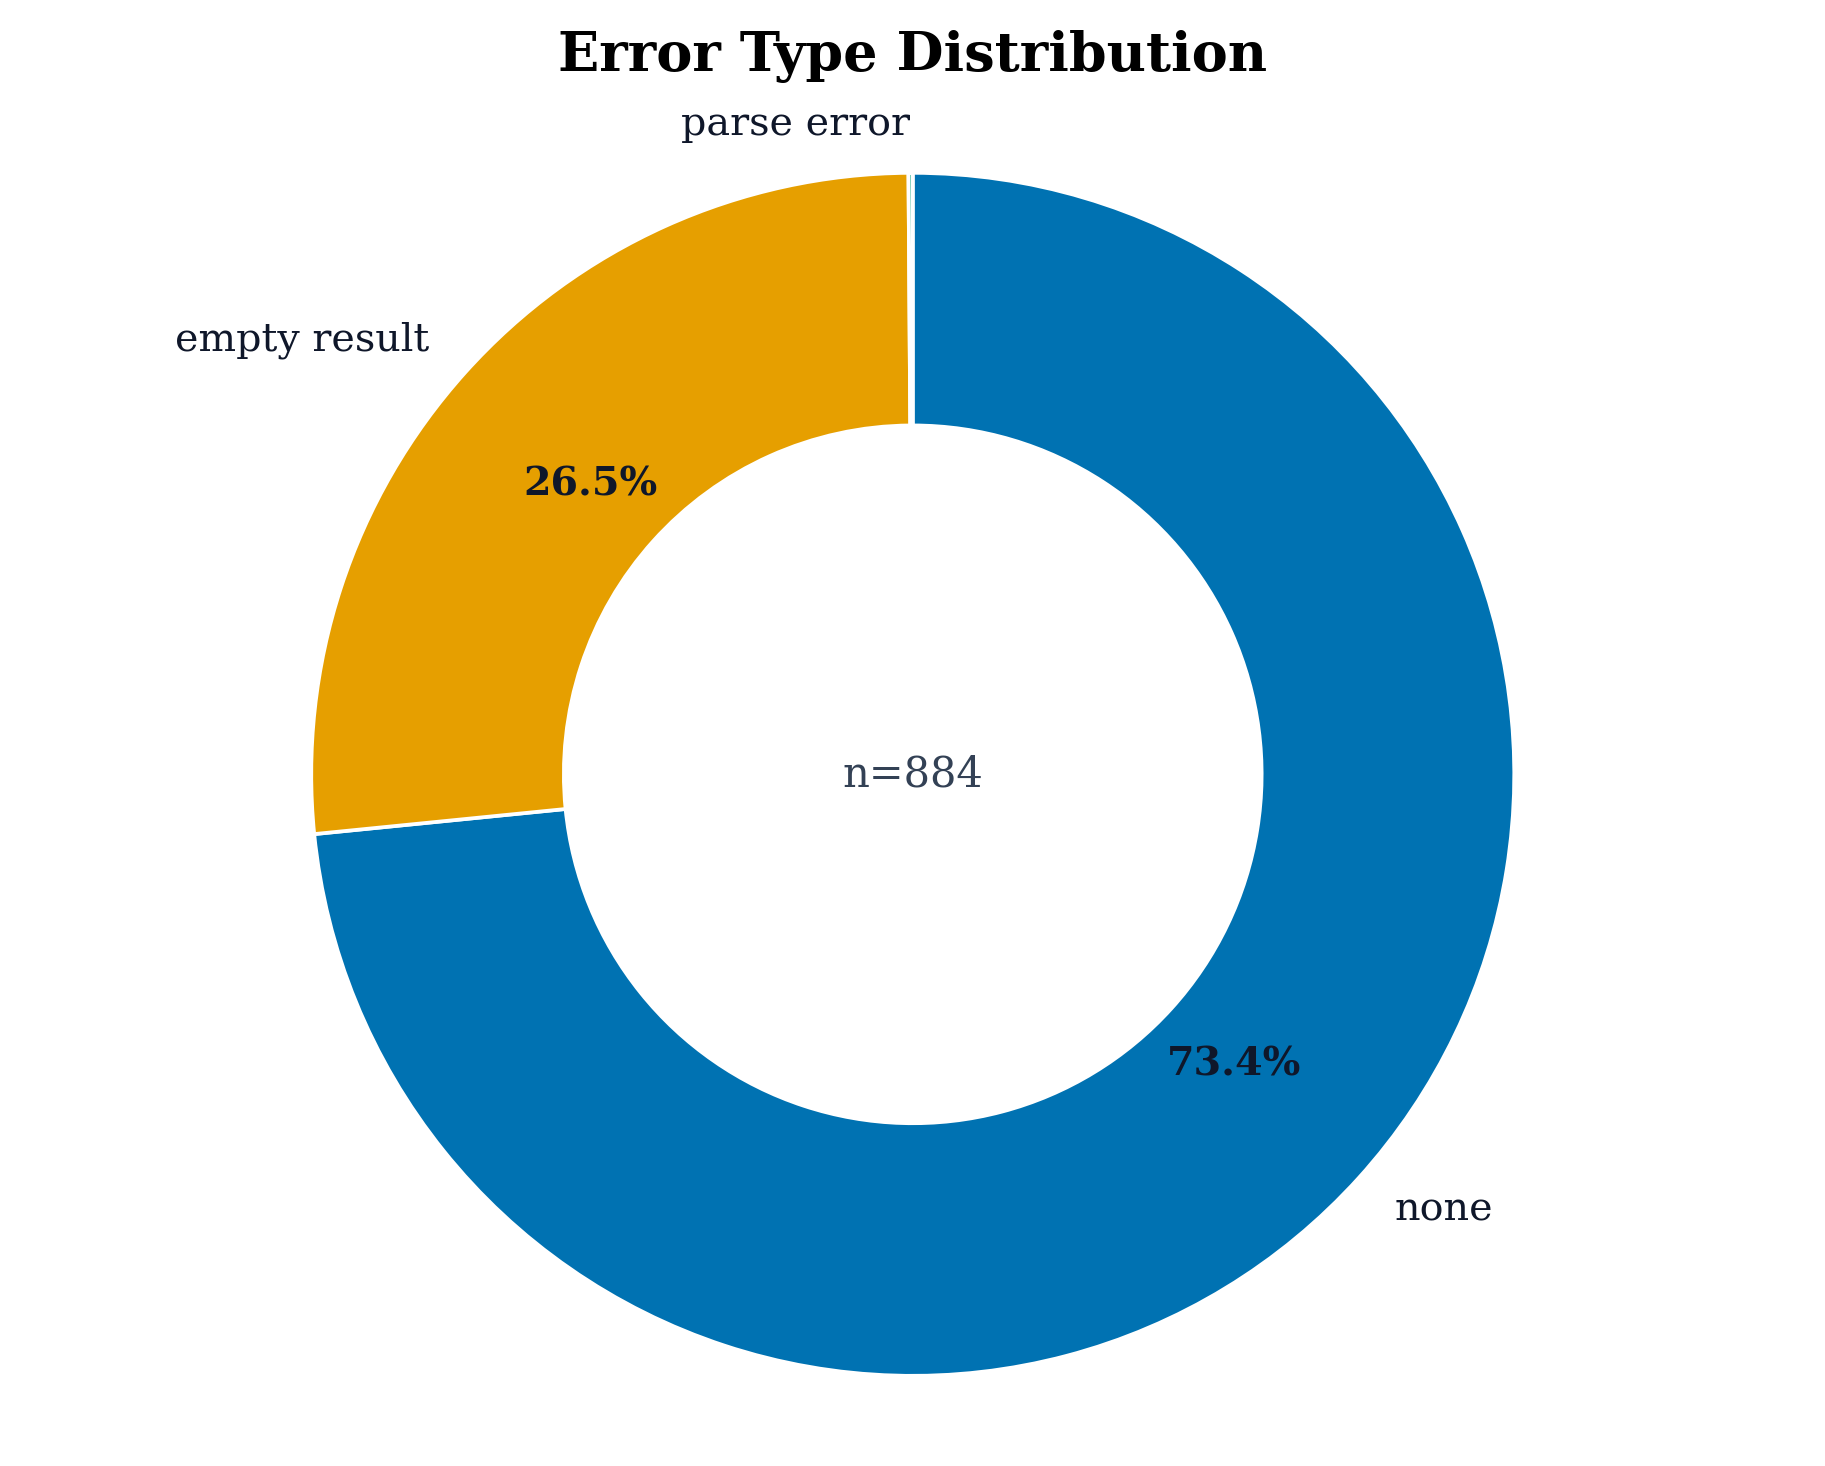
\includegraphics[width=0.85\linewidth]{figures/error_type_pie.png}
  \caption{Error type distribution across phases.}
  \label{fig:error_types}
\end{figure}

\begin{figure}[h]
  \centering
  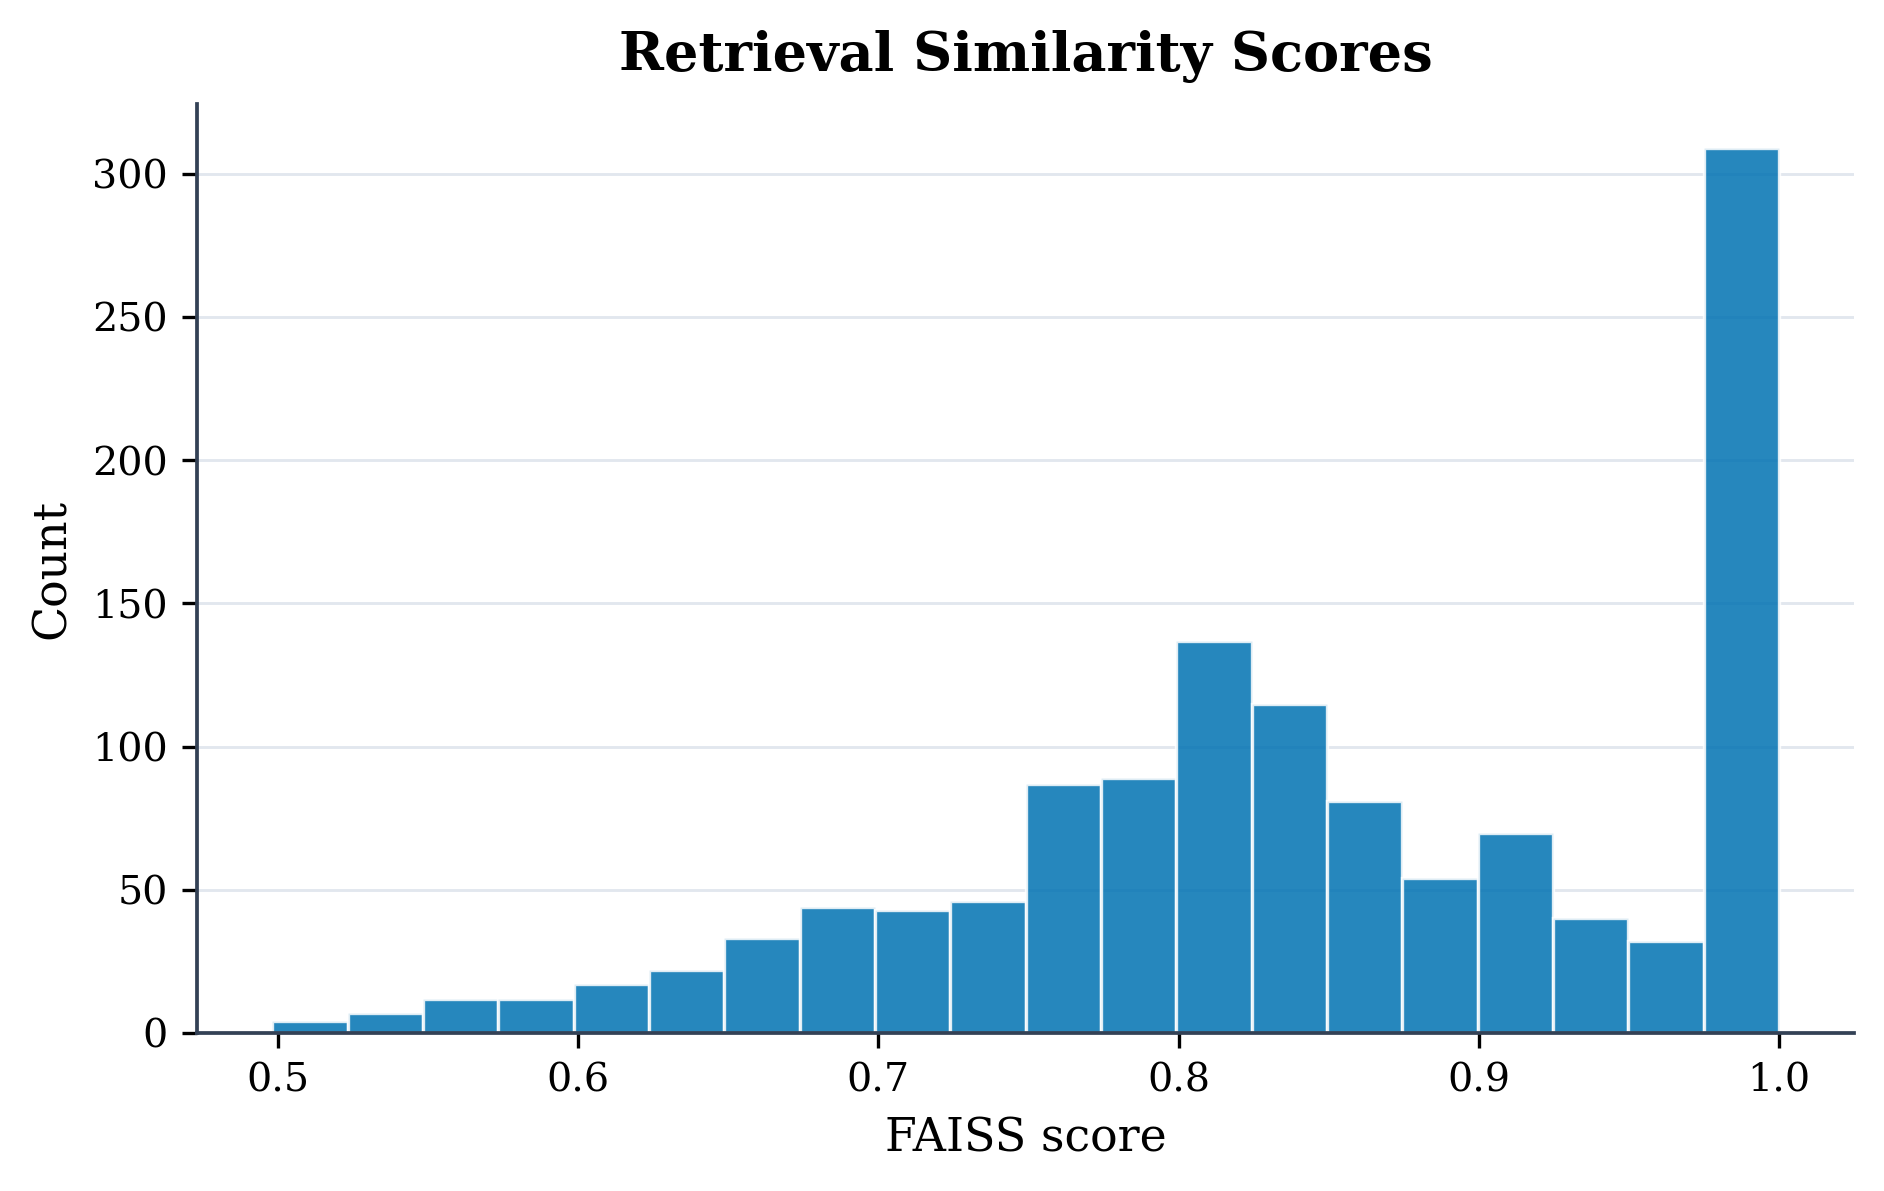
\includegraphics[width=0.95\linewidth]{figures/retrieval_scores_hist.png}
  \caption{Distribution of retrieval similarity scores.}
  \label{fig:retrieval_scores}
\end{figure}

\begin{figure*}[h]
  \centering
  \begin{minipage}{0.48\linewidth}
    \centering
    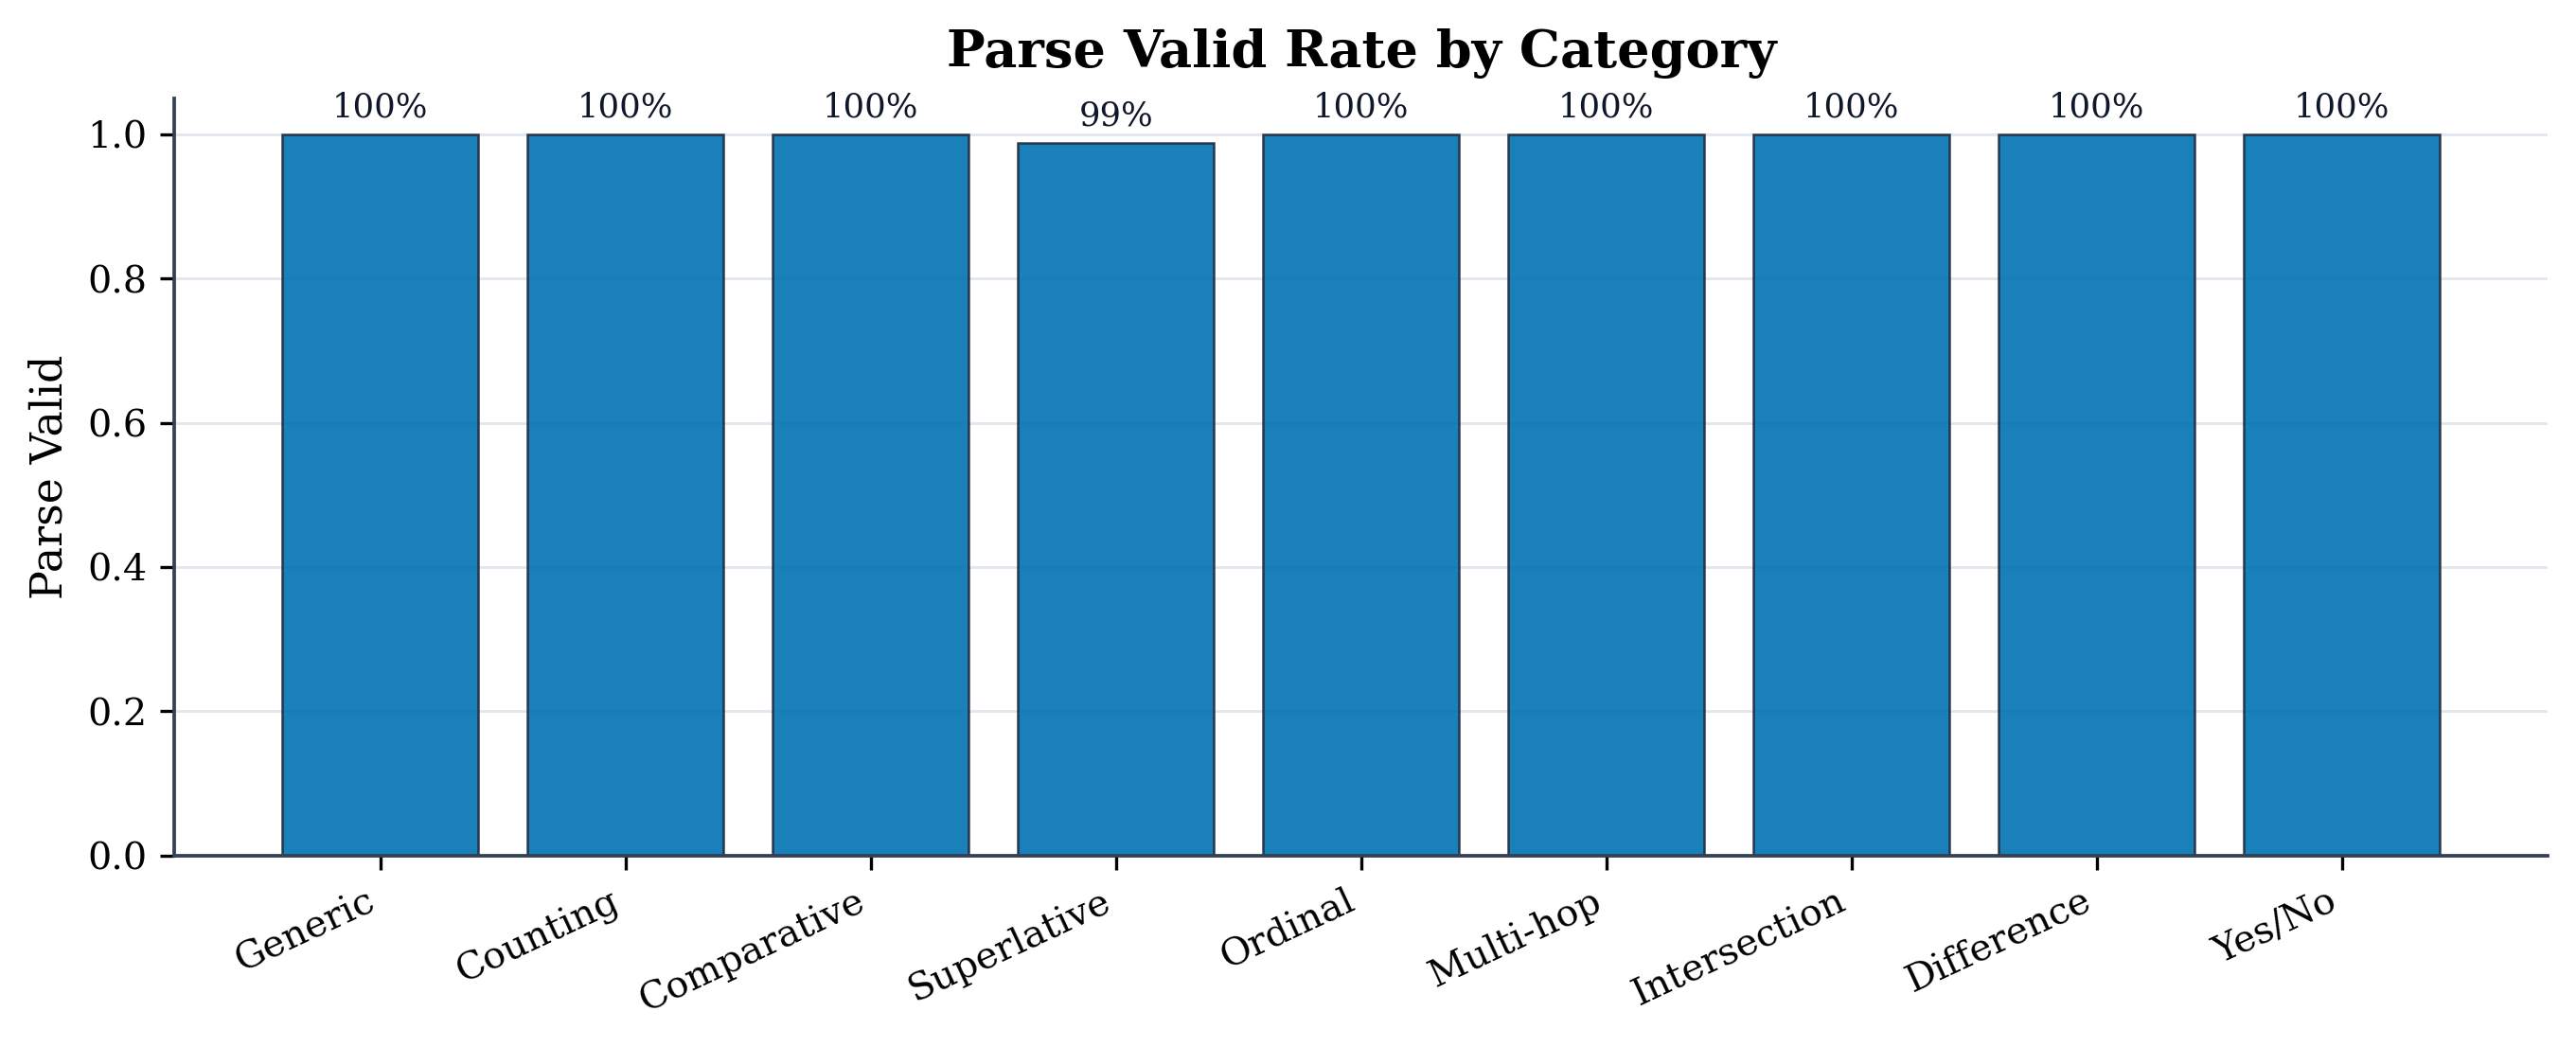
\includegraphics[width=\linewidth]{figures/parse_valid_by_category.png}
  \end{minipage}\hfill
  \begin{minipage}{0.48\linewidth}
    \centering
    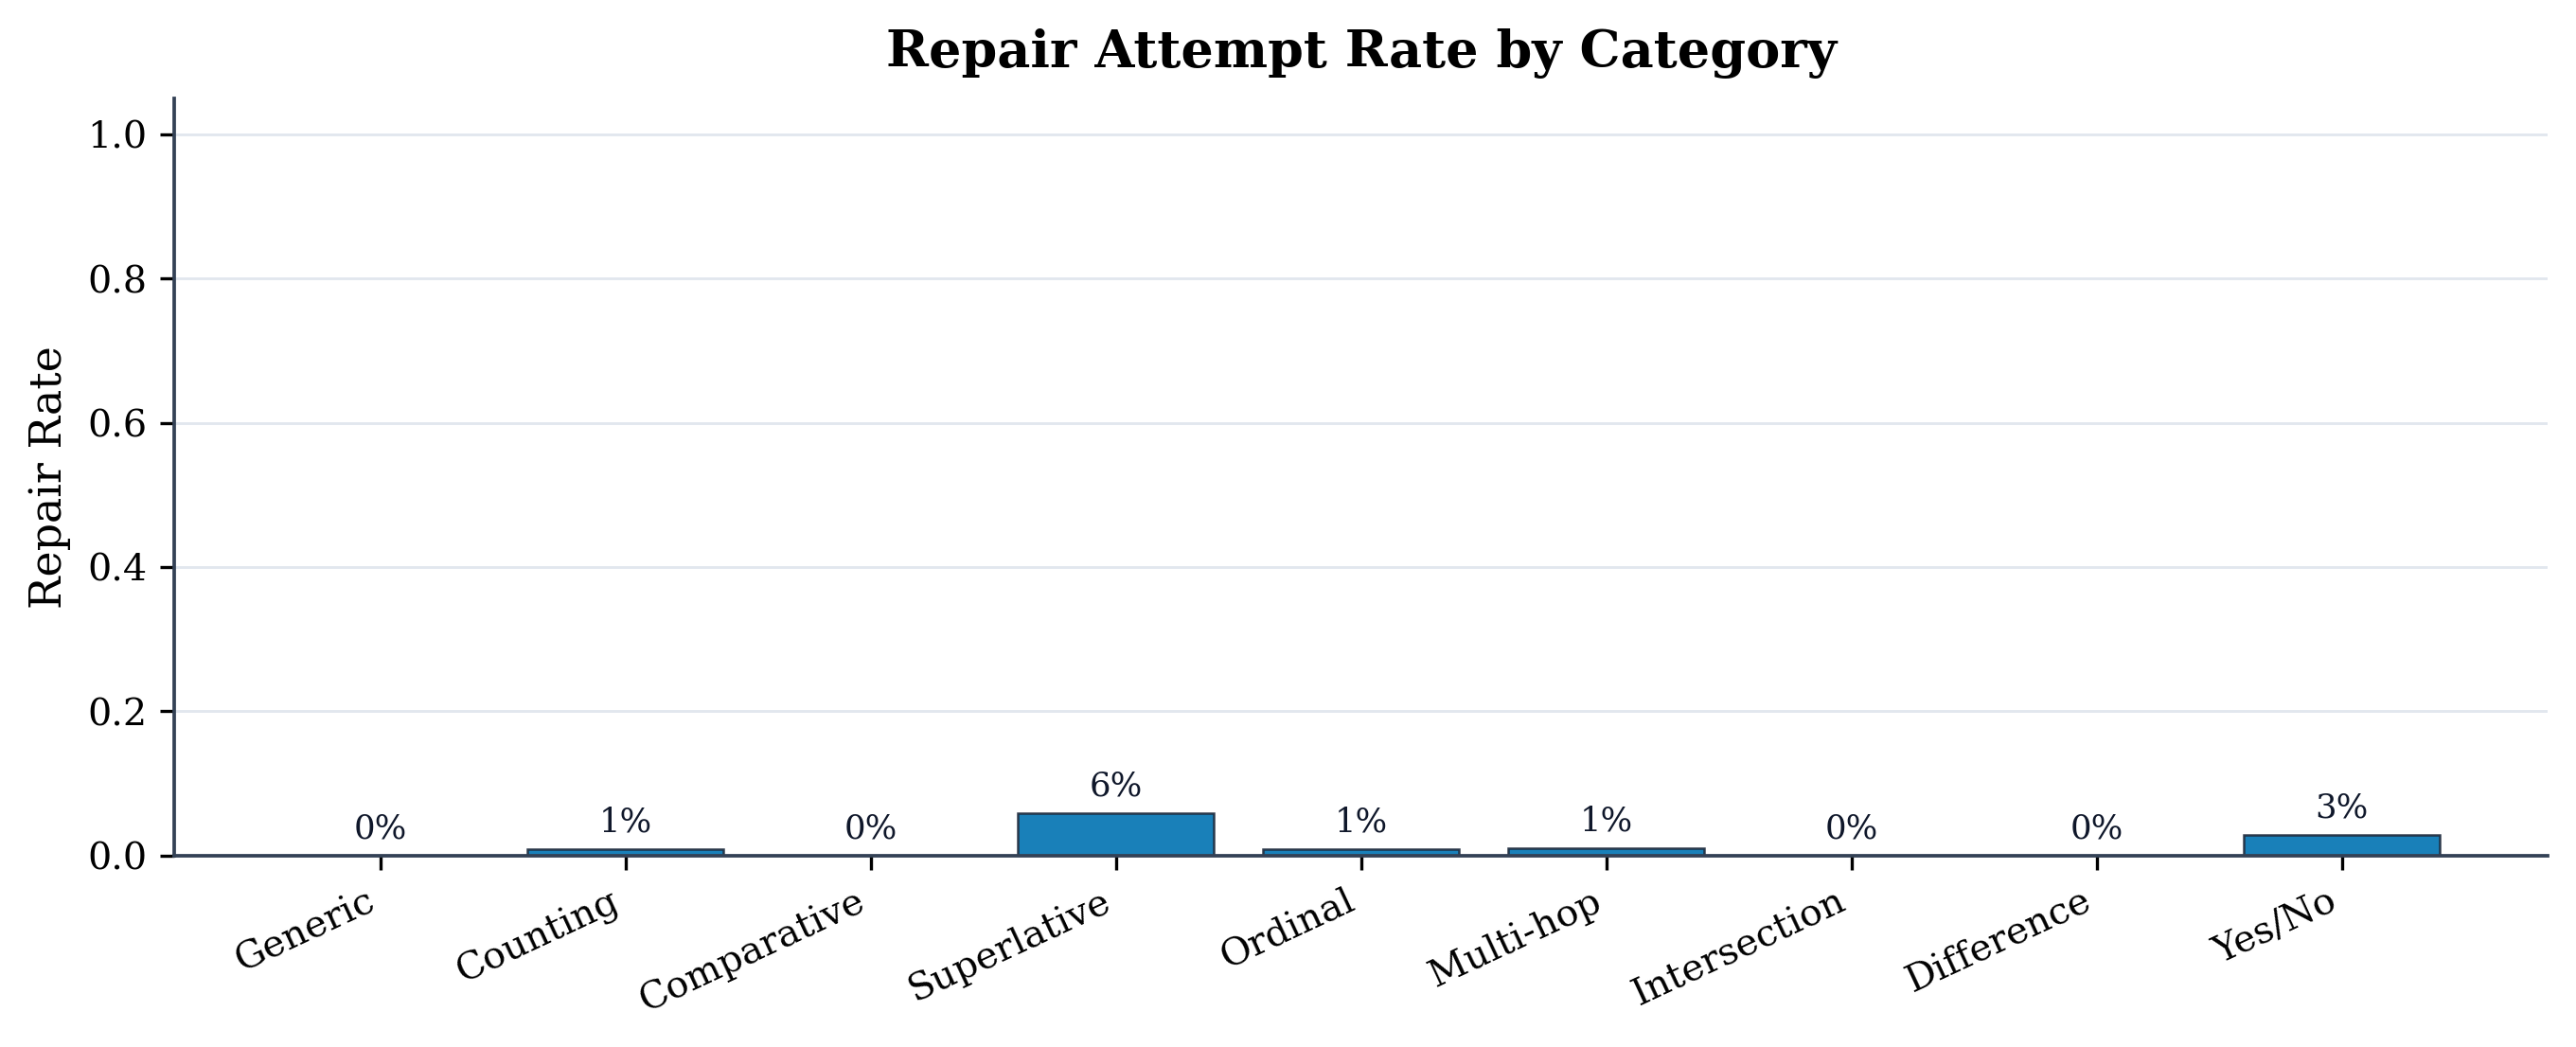
\includegraphics[width=\linewidth]{figures/repair_rate_by_category.png}
  \end{minipage}
  \caption{(Left) Parse validity by category. (Right) Repair rate by category.}
  \label{fig:parse_repair}
\end{figure*}

\begin{figure*}[h]
  \centering
  \begin{minipage}{0.48\linewidth}
    \centering
    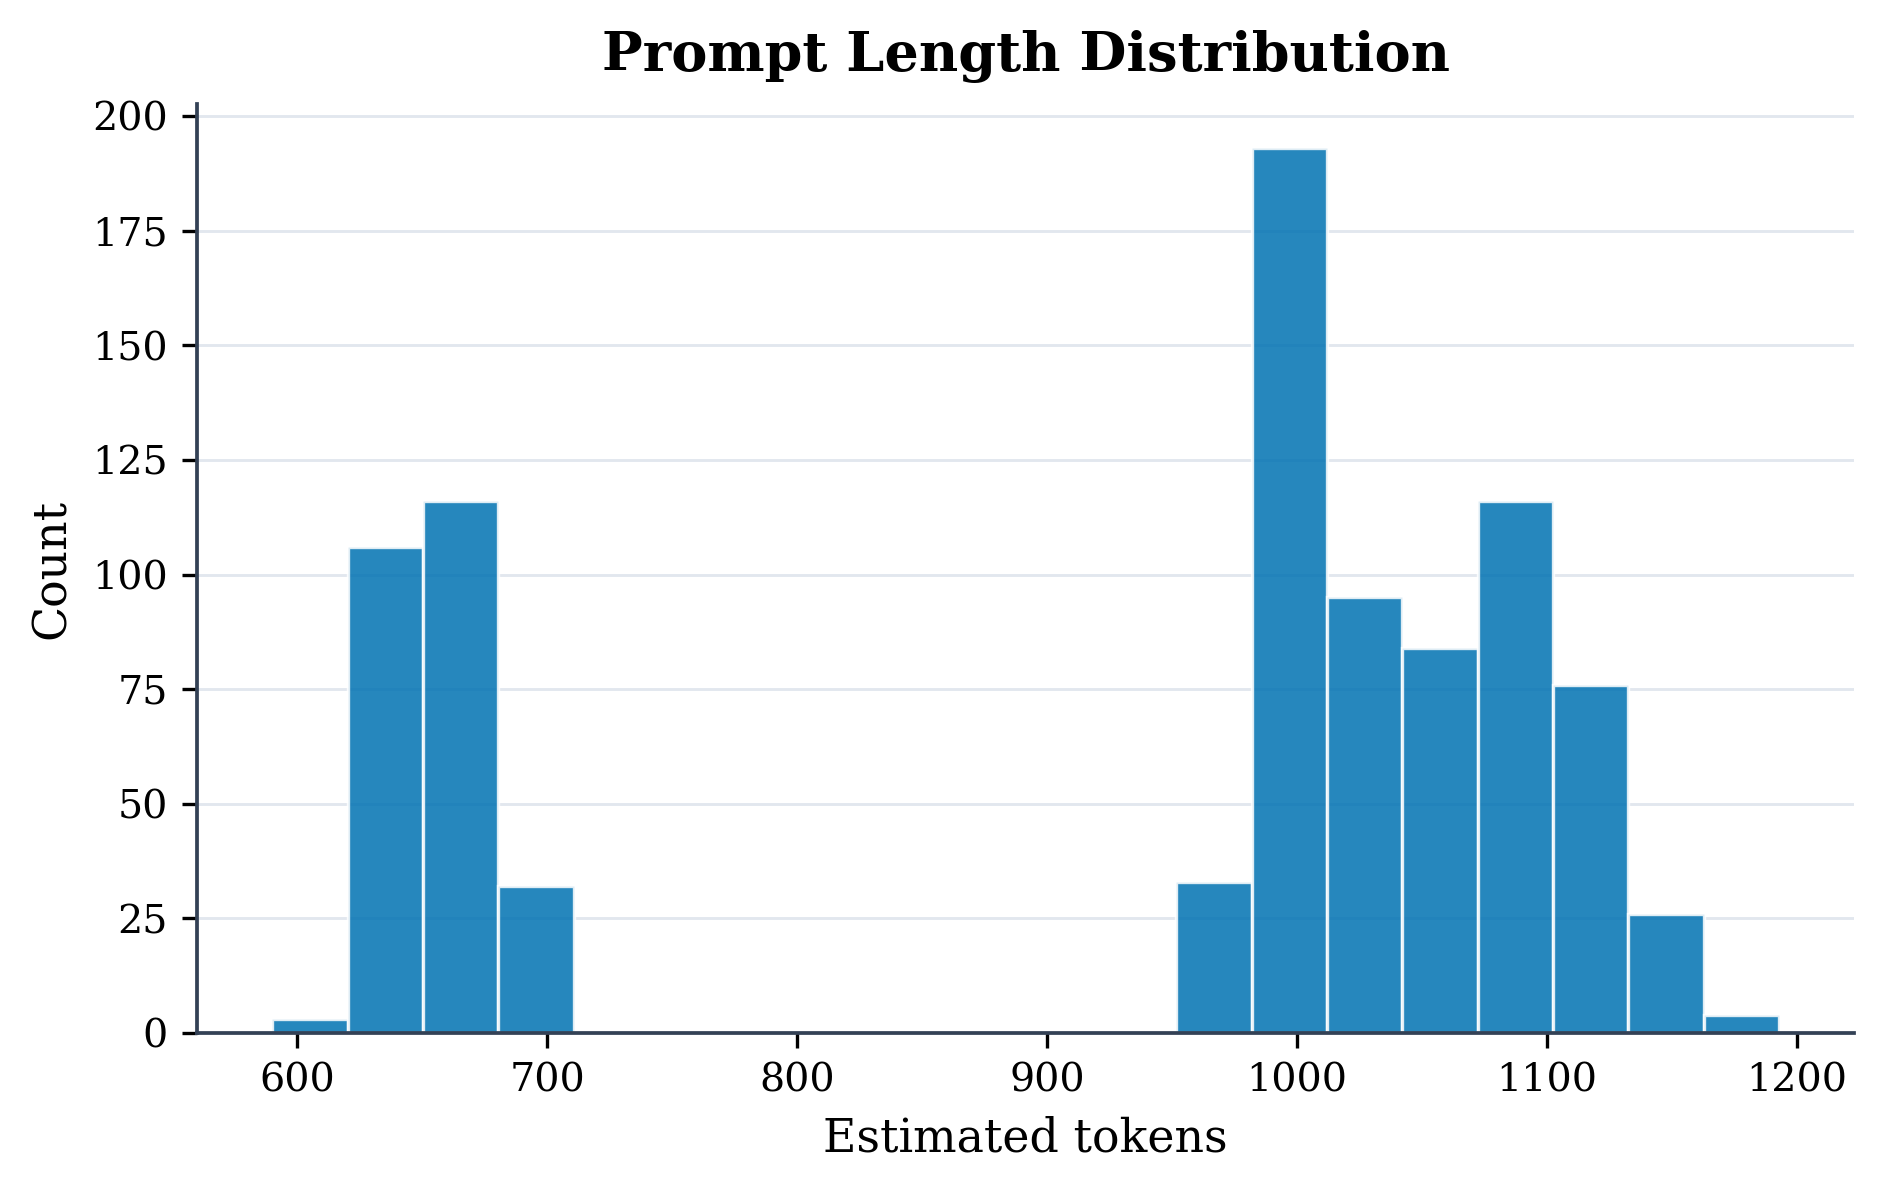
\includegraphics[width=\linewidth]{figures/prompt_length_hist.png}
  \end{minipage}\hfill
  \begin{minipage}{0.48\linewidth}
    \centering
    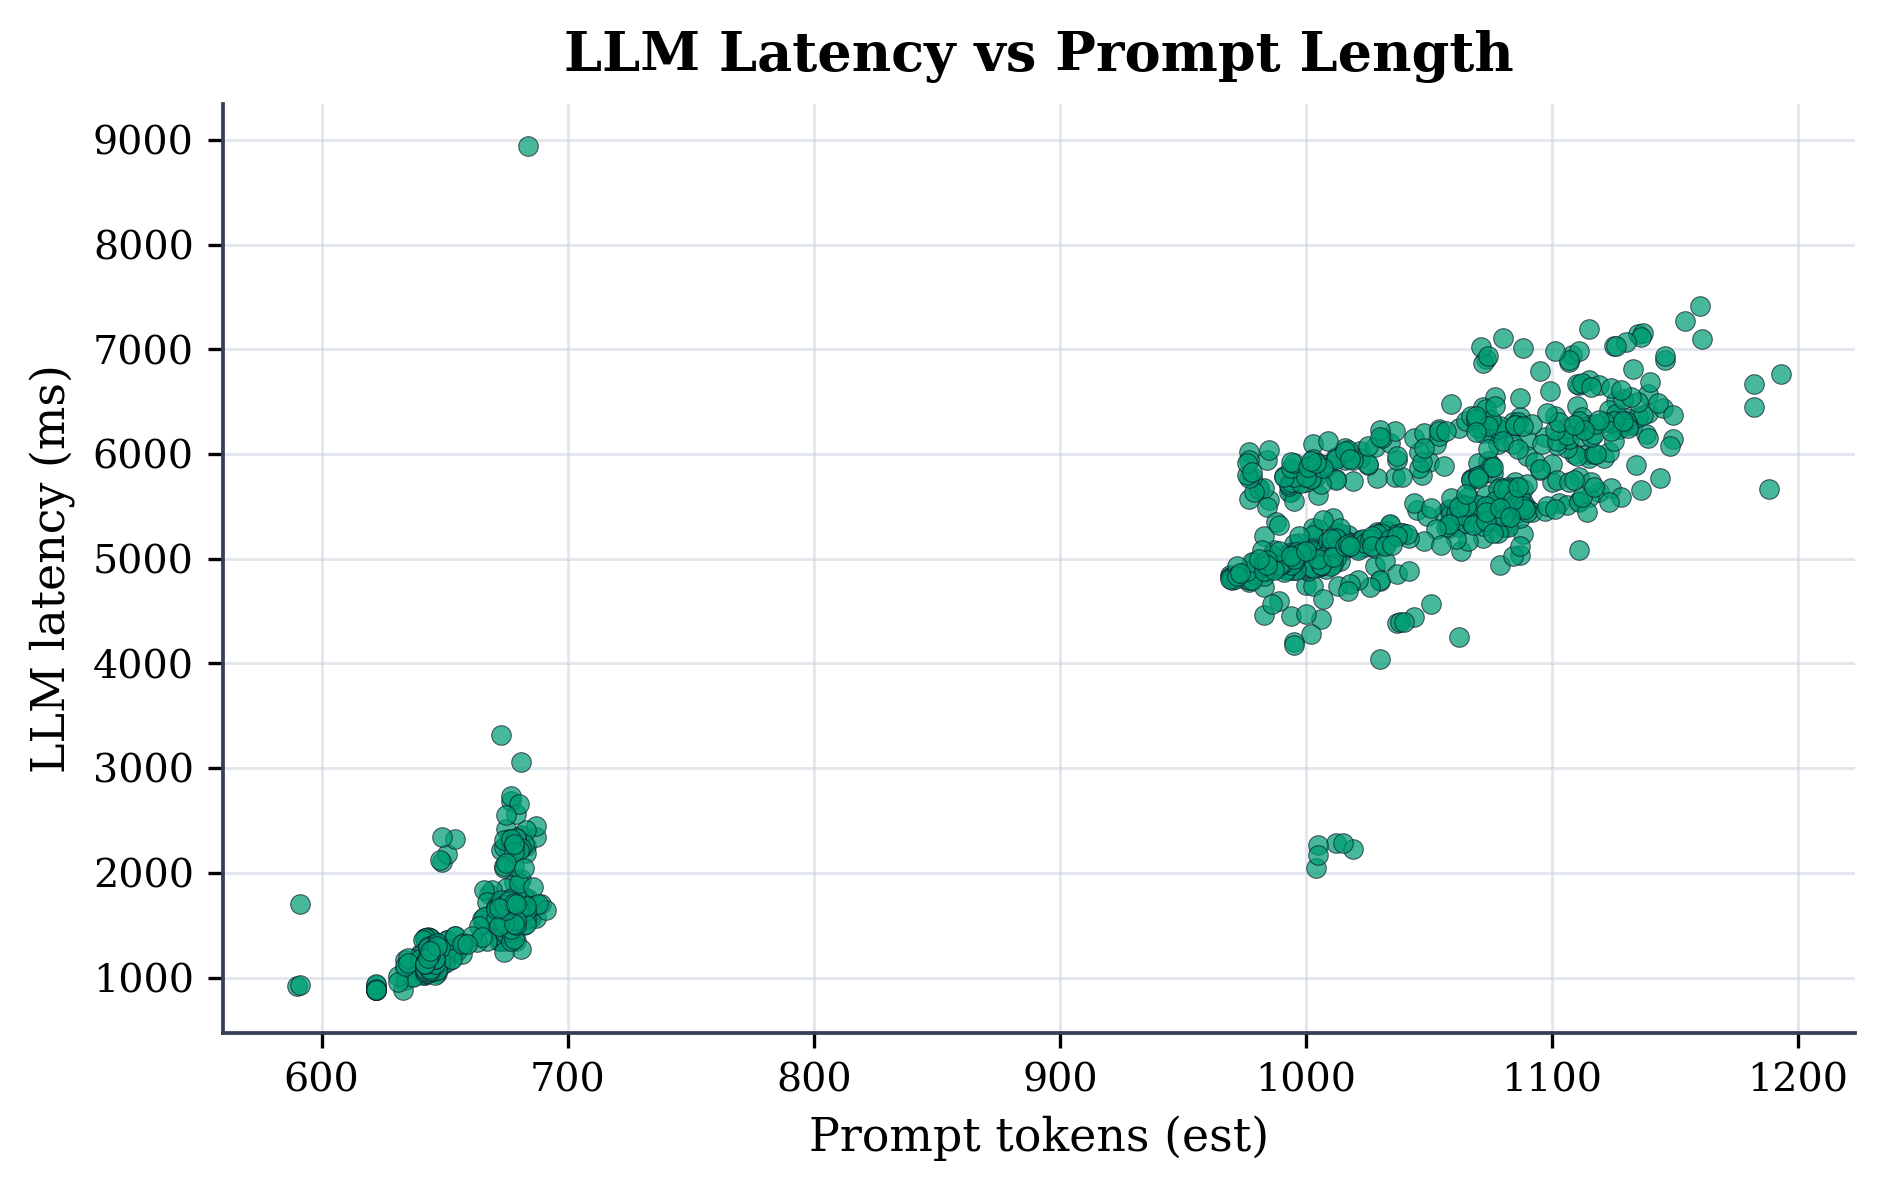
\includegraphics[width=\linewidth]{figures/llm_latency_vs_prompt.png}
  \end{minipage}
  \caption{Prompt length distribution and latency vs. prompt length.}
  \label{fig:prompt_latency}
\end{figure*}

\section{Example NL--SPARQL Pairs}
We include one example per category from the Phase 3 benchmark. Prefix declarations are omitted for brevity.

\noindent\textbf{Generic.} Q: Who is a key person at (Company: Volkswagen)?
\begin{SPARQL}
SELECT ?name
WHERE {
  VALUES ?company { <http://dbpedia.org/resource/Volkswagen> }
  ?company rdf:type dbo:Company .
  ?company dbo:keyPerson ?person .
  ?person rdf:type foaf:Person .
  ?person foaf:name ?name .
}
LIMIT 5
\end{SPARQL}

\noindent\textbf{Counting.} Q: How many companies are located in (Location: Menlo Park, California)?
\begin{SPARQL}
SELECT (COUNT(DISTINCT ?company) AS ?count)
WHERE {
  VALUES ?location { <http://dbpedia.org/resource/Menlo_Park,_California> }
  ?company a dbo:Company .
  ?company dbo:location ?location .
  ?location a gn:Feature .
}
\end{SPARQL}

\noindent\textbf{Comparative.} Q: Do (Company: Airbus) and (Company: FileMaker Inc.) have different numbers of employees?
\begin{SPARQL}
ASK {
  VALUES ?company1 { <http://dbpedia.org/resource/Airbus> }
  VALUES ?company2 { <http://dbpedia.org/resource/FileMaker_Inc.> }
  ?company1 a dbo:Company .
  ?company2 a dbo:Company .
  ?company1 dbo:numberOfEmployees ?n1 .
  ?company2 dbo:numberOfEmployees ?n2 .
  FILTER (xsd:integer(?n1) != xsd:integer(?n2))
}
\end{SPARQL}

\noindent\textbf{Superlative.} Q: Which company has the most employees?
\begin{SPARQL}
SELECT ?company ?employees
WHERE {
  ?company a dbo:Company .
  ?company dbo:numberOfEmployees ?employees .
}
ORDER BY DESC(xsd:integer(?employees)) ?company
LIMIT 1
\end{SPARQL}

\noindent\textbf{Ordinal.} Q: Which company was founded second earliest?
\begin{SPARQL}
SELECT ?company ?year
WHERE {
  ?company a dbo:Company .
  ?company dbo:foundingYear ?year .
}
ORDER BY ASC(xsd:integer(?year)) ?company
OFFSET 1
LIMIT 1
\end{SPARQL}

\noindent\textbf{Multi-hop.} Q: Which location contains companies that have a key person?
\begin{SPARQL}
SELECT DISTINCT ?location
WHERE {
  ?company a dbo:Company .
  ?company dbo:keyPerson ?person .
  ?person rdf:type foaf:Person .
  ?company dbo:location ?location .
  ?location a gn:Feature .
}
LIMIT 5
\end{SPARQL}

\noindent\textbf{Intersection.} Q: Which companies are located in (Location: California) and are in the (Industry: Software)?
\begin{SPARQL}
SELECT DISTINCT ?company
WHERE {
  ?company a dbo:Company .
  ?company dbo:location <http://dbpedia.org/resource/California> .
  ?company dbo:industry <http://dbpedia.org/resource/Software> .
}
LIMIT 5
\end{SPARQL}

\noindent\textbf{Difference.} Q: Are (Company: Airbus) and (Company: FileMaker Inc.) in different industries?
\begin{SPARQL}
ASK {
  VALUES ?company1 { <http://dbpedia.org/resource/Airbus> }
  VALUES ?company2 { <http://dbpedia.org/resource/FileMaker_Inc.> }
  ?company1 a dbo:Company .
  ?company2 a dbo:Company .
  ?company1 dbo:industry ?industry1 .
  ?company2 dbo:industry ?industry2 .
  FILTER (?industry1 != ?industry2)
}
\end{SPARQL}

\noindent\textbf{Yes/No.} Q: Is (Company: Facebook) located in (Location: California)?
\begin{SPARQL}
ASK {
  <http://dbpedia.org/resource/Facebook> a dbo:Company ;
    dbo:location <http://dbpedia.org/resource/California> .
}
\end{SPARQL}

\end{document}
